\section{The b-tagging performance in Run II}\label{sec:Pix_performance}
%\pagestyle{plain}
\subsection{Physics motivation}
The identification of jets originating from bottom quarks (denoted as b-tagging in the following) is an important ingredient for the high \pt physics program planned for the ATLAS experiment, since many interesting physics process contain bottom quarks in the final state, while the most abundant backgrounds contains mostly up, down and strange quarks or gluon jets.
The reason of this interest is that b-quarks are the heaviest quarks in the Standard Model which still form hadrons before undergoing a weak decay, contrary to what happens for the top quark, the heaviest quark in the Standard Model, which can be detected only indirectly by analyzing their decay products (in most cases a bottom quark and an additional W).
\begin{figure}
\centering
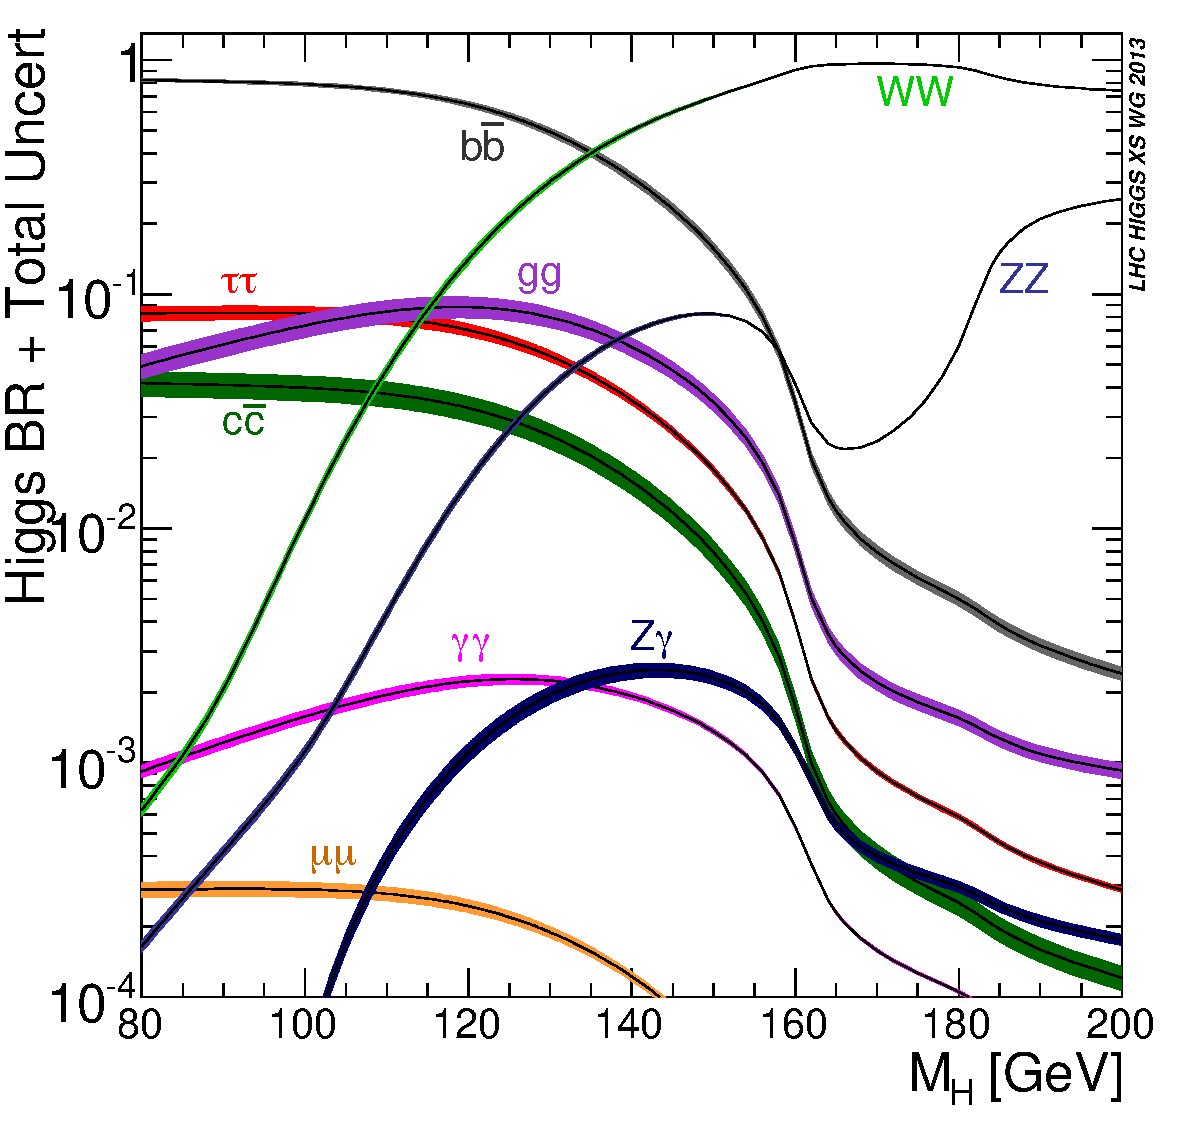
\includegraphics[width=0.5\textwidth]{Images/b-tagging/Higgs_BR_LM.pdf}
\caption{Standard Model Higgs boson decay branching ratios}
\label{pic:higgs_br}
\end{figure}
The aim of the b-tagging is therefore to extract the b-quark with high jet efficiency, while rejecting most of the background contamination from jets originating from fragmentation of light (u and s) quarks, gluons and c-quarks.
B-tagging is also crucial for the study of the Higgs-boson properties given the fact that its favorite decay channel is $H\rightarrow b\overline{b}$, as it can be seen in figure~\ref{pix:higgs_br}.\\
From the physics point of view the hadronization of b-quarks has several unique properties, which can be exploited by b-tagging.
A b-quark, once produced, fragments necessarily into a b-flavored hadron, like a B* or a B**, which decays immediately, strongly or electromagnetically, into a ground state b-hadron plus one or more further particles, while in the remaining cases a ground state b-hadron is produced.
\begin{table}
\begin{center}
\begin{tabular}{|c|c|}
\hline
b-hadron 	& Branching fraction \\
\hline
$B^+$			& $(40.0\pm1.2)\percent$ \\
$B^0$			& $(40.0\pm1.2)\percent$ \\
$B^0_S$			& $(11.4\pm2.1)\percent$ \\
$b-baryon$	& $(8.6\pm2.1)\percent$ \\
\hline
\end{tabular}
\caption{Branching fraction of b-hadrons produced out of the fragmentation of b-quarks. Taken from \cite{Giac_71}}
\label{tab:b_br}
\end{center}
\end{table}
From an experimentalist perspective, one is however only interested in the transition from a b-quark into the final ground state b-hadron, since the timescale typical for electromagnetic and strong interactions is so small that the B* and the B** decay vertices are not significantly displaced withe respect to the primary vertex. The various different fractions of ground state b-hadrons produced out of the fragmentation of an original b-quark are presented in table \ref{tab:b_br}.
The fragmentation function describes the distribution of the fraction of energy of the original b-quarks which is kept by the b-hadron. Due to the b-quark fragmentation function being very hard, most of the original b-quark energy is transmitted to the final b-hadron: this fraction is for example on average $\simeq$70\percent for b-quarks with a momentum of $\simeq \SI{45}{\GeV}$. This property cab be exploited during b-tagging, since the fragmentation function for light-quarks into light hadrons or c-quarks into -hadrons is softer.
%Any of the finally produced b-hadrons decay through weak interactions and therefore have a significant lifetime, which is on average, for all the b-hadrons considered, 
The Effective distance traveled in the detector by the b-hadron before decaying depends on the b-hadron momentum, which enters the relativistic boost factor $\beta\gamma$. This means that a b-hadron with a momentum of 50 GeV will travel around $3\milli\meter$, which is a visible flight length in the detector. Due to the combination of the b-hadron lifetime and relatively high mass ($m_B\simeq\SI{5.28}{\GeV}$), which results in a non-negligible decay angle of the b-hadron decay products with respect to the b-hadron flight direction, the charged particles produced at the decay vertex will be on average significantly displaced with respect to the primary vertex position.\\
This is the main signature which is exploited by $lifetime$ based b-tagging algorithms, which are based either on the presence of significantly displaced tracks, as in impact parameter based b-tagging algorithms, or on the explicit reconstruction of the b-hadron decay vertex, as in secondary vertex based b-tagging algorithms.
Weak decays are governed by the CKM matrix mechanism \cite{Giac_72} and \cite{Giac_73}: since $|V_{cb}|^2 >> |V_{ub}|^2$ b-hadrons decay preferably into a c-hadron plus additional particles. These c-hadrons can be again excited states, like D* and D**, but these again decay with negligible lifetime to weakly decaying c-hadrons.
The c-hadrons can still travel for a significant path in the detector and form with its decay products a visible tertiary vertex, displaced with respect to both secondary and primary vertices.
There are several possible strategies to deal with such tertiary from c-hadron decays. In the case of the b-tagging algorithms based purely on impact parameter information from the charged particle tracks, the presence of tracks with a more significant displacement does not require an explicit strategy: these tracks will in general just improve the b-tagging performance.Their presence is taken into account when the algorithm is calibrated using Monte Carlo simulated events or as soon as the amount collected data will allow it directly with data.
Another property which is usually exploited by b-tagging is the fraction of b and c-hadron decays into lepton, a lepton from the semi-leptonic decay of a b-hadron or from the subsequent decay of the c-hadron turns out to be produced in a b-quark in the $\simeq$21\percent of the cases. This is valid for muons and electrons, which brings the overall fraction to $\simeq$42\percent. Due to the b or c-hadron mass, the lepton will be emitted with an average transverse momentum comparable with $m_{bHad}$ or $m_{cHad}$. By identifying either an electron or a muon originating from a jet and by requiring it to have a sufficiently high transverse momentum with respect to the jet axis, it is possible to identify b-jets, rejecting light jets, where leptons are expected mainly from the in-flight decay of charged pions and kaons, from Dalitz decays of neutral pions, from $\gamma$-conversion or from misidentified leptons.
%The most interesting physics cases addressed by this selection involve events with final states containing more than one b-jet. This event class is specially relevant for the Higgs-boson, for which the decay in $b\xoverline{b}$ is the dominant channel. Final states containing hadronic jets have large backgrounds at hadron colliders thus, even if the production rate is lower, events with a Standard Model Higgs boson produced in association with other particles present a significantly better signal to noise ratio.
%Among these topologies, the $H \rightarrow b\xoverline{b}$ channel where the Higgs boson is produced by way of the associated production channel ttH is characterized by a large number of b-jets in the final state and the signal acceptance can be uniquely enhanced by requesting b-tagging triggers firing. Similar signatures, in supersymmetric theories, which again benefit from this class of triggers are the channels bbH, bbA with H/A → bb or H → hh → bbbb. A study to quantify the on-line selection efficiency for the benchmark signal ttH is presented in Chapter 8.
%Another important use case of on-line b-tagging is the selection of fully hadronic tt events. This topology is taken as the benchmark sample for events with two b-jets in the final state and efficiency comparing the jet and the b-jet triggers are reported again in Chapter 8.
%The b-tagging selection, i.e. the identification of jets stemming from the fragmentation and hadronization of b quarks, takes advantages of several physical properties which allow the separation of them from jets containing only lighter quarks. The properties of B hadrons upon which the b-jet identification may rely are:
\subsection{The Run II b-tagging algorithm}
The basic b-tagging algorithms use charged particle tracks to produce a set of variables which discriminate between different jet flavor. Tracks are first associated to a jet and are then required to pass a quality selection. ATLAS uses three distinct basic b-tagging algorithms, which provide complementary information
\begin{itemize}
\item Impact parameter based algorithm
\item Inclusive secondary vertex reconstruction algorithm
\item Decay chain multi-vertex reconstruction algorithm
\end{itemize}
The output of these b-tagging algorithms are later combined in a multivariate discriminant which provides the best separation between the different jet flavors.
\subsubsection{Track Selection}
Tracks are associated to calorimeter jets based on their angular separation $\Delta R(track,jet)$. The $\Delta$ association requirement varies as a function of the jet pT , resulting in a narrower cone for jets at high pT which are more collimated. A given track is associated with only one jet; if it satisfies the association criterion with respect to more than one jet, the jet with the smallest $\Delta R$ is chosen.
The track selection depends on each specific b-tagging algorithm. For the impact parameter based algorithm, a tight selection is applied. The most important requirements include a requirement on the track \pt above 1 GeV, the transverse and longitudinal impact parameters to be limited to $|d_0| < 1 \milli\meter$ and $|z0 × sin\theta|<1.5\milli\meter$, and at least two hits in the pixel detector. For the secondary vertex based algorithms a looser selection is used, relying on the secondary vertex reconstruction to provide additional purity. This includes requiring track \pt to be above $700-800~MeV$ and significantly looser requirements in terms of impact parameter and track quality.
\subsubsection{Impact Parameter based Algorithms: IP2D, IP3D}
The IP2D and IP3D algorithms \cite{BTAG_15}, make use of the signed impact parameter significance of the tracks matched to the jet.
In this case the sign of the impact parameter is a lifetime information associated to the impact parameter, replacing the sign od the geometrical definition of the impact parameter. The sign is defined positive (negative) if the point of closest approach of the track to the primary vertex is in front (behind) the primary vertex with respect to the jet direction.
\begin{figure}
\centering
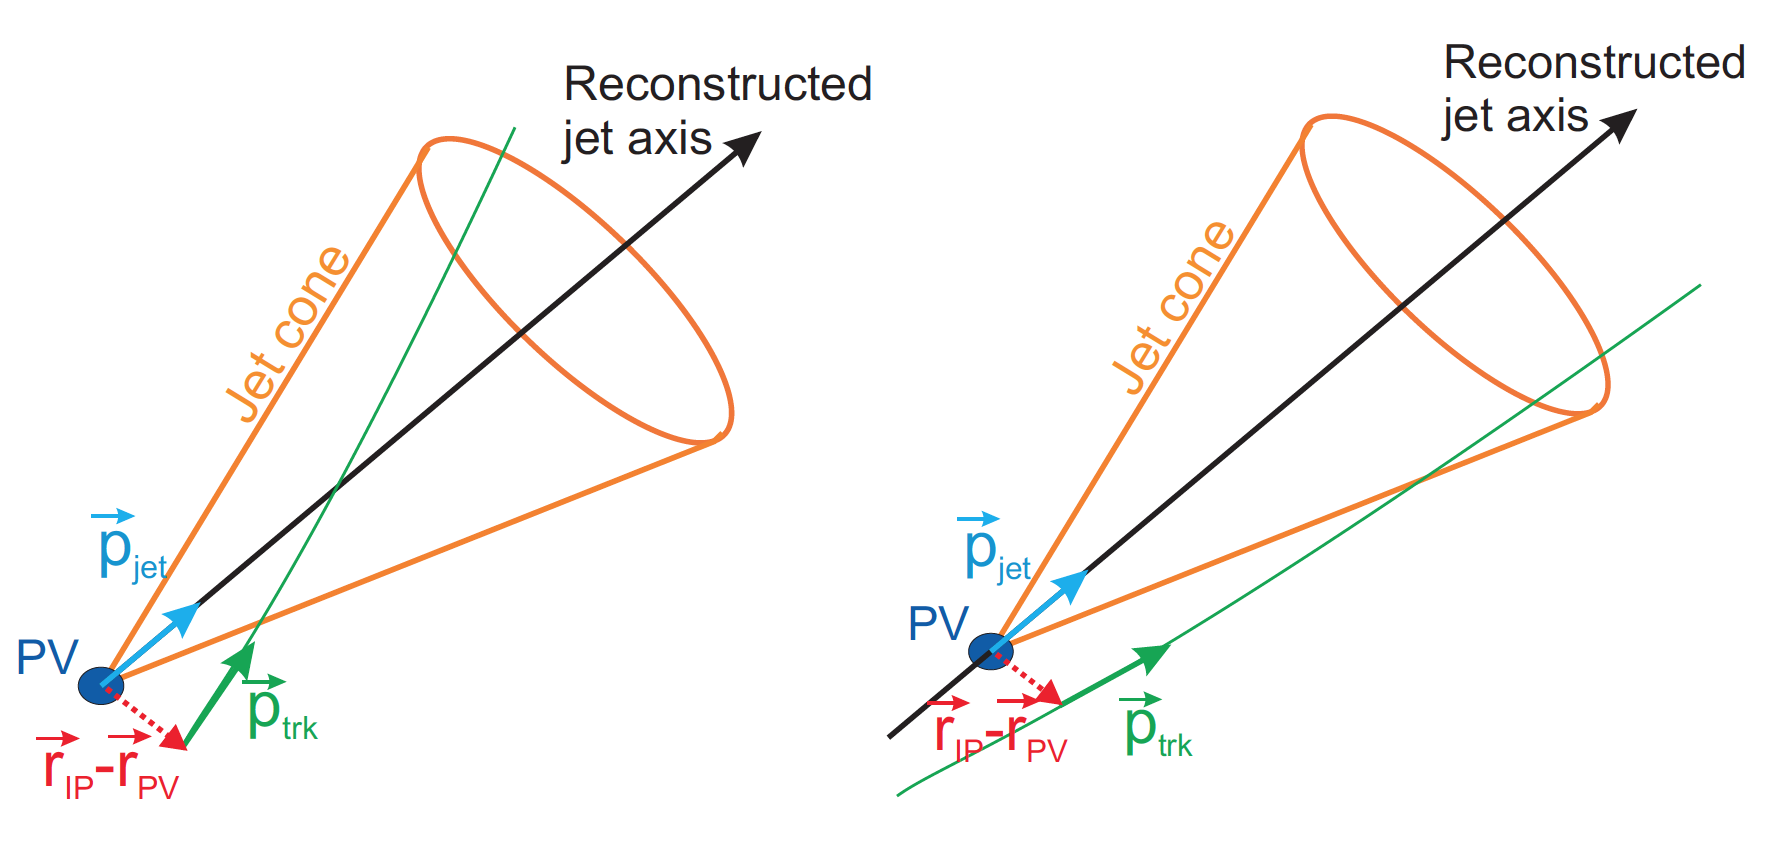
\includegraphics[width=0.9\textwidth]{Images/b-tagging/ipxd_sign.png}
\caption{Definition of variables needed to compute the lifetime sign of a track in the three-dimensional space. In addition a positive (left) and negative lifetime track is shown.}
\label{pic:ipxd_sign}
\end{figure}
Both cases are illustrated in Figure \ref{pic:pxd_sign}, together with the variables needed to define the lifetime sign.
The vector $\Delta\vv{r}_{IP} = \vv{r}_{IP} - \vv{r}_{PV}$ defines a three-dimensional impact parameter of the track momentum defined at the point of closest approach to the primary vertex.
The lifetime sign can then be defined in the three-dimensions, according to the variables $\vv{p}_{jet}$, $\vv{p}_{trk}$ and $\Delta\vv{r}_{IP}$:
\begin{equation}
sign_{3D} = sign([\vv{p}_{trk} \times \vv{p}_{jet}] \cdot [\vv{p}_{trk} \times \Delta\vv{r}_{IP}])
\end{equation}
or it can be alternatively defined on the transverse plane ($x-y$) pr on the longitudinal plane ($r\phi-z$) by considering the projection of the three-dimensional impact parameter on those planes. In these cases the formula simplifies and the lifetime signs can be expressed as:
\begin{equation}
sign_{r\phi} = sign(sin(\phi_{jet} - \phi_{trk})\cdot d_{0,trk}),\\
sign_{z} = sign(sin(\eta_{jet} - \eta_{trk})\cdot d_{0,trk}).\\
\end{equation}
The computation of the lifetime sign assumes that the jet direction reproduces, up to a good approximation, the b-hadron direction: from the physical point of view this assumption can only be fullfilled in a approximate way, since the jet momentum is supposed to reproduce the momentum of the initial quark, which is given by the sum of the momentum of the b-hadron and of the remaining tracks arising directly from fragmentation. Under this assumption and up to resolution effects both on jet direction and on the impact parameter and momentum of the track, the lifetime sign fro tracks originating from b-hadron decays is positive.
The extension of the impact parameter significance distribution to high values for $K^0_S$ decays and conversions are limited by applied impact parameters cuts.

The impact parameter significances of all N tracks associated to the jet to tag need to be combined into a single discriminating variable. It is assumed that the tracks are uncorrelated, so that their probability density functions (PDF) are uniquely defined as a function of the jet flavor. Using a likelihood function defined according to the product of these PDFs, under the hypothesis of uncorrelated tracks, the following likelihood ratio provides optimal separation, according to the Neyman-Parson lemma:
\begin{equation}
LR(IP_1,IP_2,...IP_N) = \frac{\Pi_{i=1}^N PDF_b(IP_i)}{\Pi_{i=1}^N PDF_l(IP_i)}
\end{equation}
For convention the discriminating variable used for b-tagging is then defined as:
\begin{equation}
weight(IP_1,IP_2,... , IP_N) = log(LR(IP_1,IP_2,...,IP_N)).
\end{equation}
Using such a formalism, wo impact parameter based b-tagging algorithms are constructed based on the definition of PDF($IP_i$);
\begin{equation}
IP2D:\quad PDF(IP_i) = PDF(IP_{i,r\phi}),\\
IP3D:\quad PDF(IP_i) = PDF(IP_{i,r\phi},IP_{i,z}).
\end{equation}
In the first case the track PDF is one-dimensional, based on the transverse impact parameter significance. In the second case it is a two-dimensional PDF, based on the transverse and longitudinal impact parameter significance.
The impact parameter based algorithm permit to obtain a very good b-tagging performance and at the same time allow to keep the method fairly simple, with a single track based PDF to be calibrated for each quark flavor.
One of the reason for the good performance is that the likelihood method based on the impact parameter significance contains implicitly, as a prior knowledge in the PDF for b-jets, the fraction of tracks expected to arise from fragmentation and the fraction expected to arise from b and c-hadron decays. However, this method has also some drawbacks. One is that the fraction of tracks from fragmentation depends on the energy of the initial quark, the second is that, while the impact parameter significances of prompt tracks is independent on the jet \pt and $\eta$, the impact parameter from secondary decays is not; in fact, while the impact parameter as such is nearly invariant under Lorentz boosts of the b-hadron, the error decreases with increasing track \pt and smaller $\eta$. The track-based PDF is thus not invariant neither under a boost of the b-quark nor under a boost of its emerging charged particles tracks. This an be cured both by making track-PDF category dependent, where the categories corresponds to different interval either in jet kinematics or in the track errors.
Using a category dependent PDF brings a significant improvement in performance,but it has the disadvantage of increasing the number of free parameters of the likelihood model and making an eventual calibration on data more difficult \cite{Giac_44}.
\begin{table}
\begin{center}
\begin{tabular}{|c|c|c|c|c|}
\hline
\# & Description & b-jets & c-jets & light jets\\
\hline
0 & No hits in first two layers; exp. hit in L0 and L1 & 1.5 & 1.6 & 1.6\\
1 & No hits in first two layers; exp. hit in L0 and no exp. hit in L1 & 0.1 & 0.1 & 0.1\\
2 & No hits in first two layers; no exp. hit in L0 and exp. hit in L1 & 0.03 & 0.03 & 0.03\\
3 & No hits in first two layers; no exp. hit in L0 and L1 & 0.03 & 0.03 & 0.02\\
4 & No hit in L0; exp. hit in L0 & 2.4 & 2.3 & 2.1\\
5 & No hit in L0; no exp. hit in L0 & 0.9 & 0.9 & 0.9\\
6 & No hit in L1; exp. hit in L1 & 0.5 & 0.5 & 0.5\\
7 & No hit in L1; no exp. hit in L1 & 2.4 & 2.4 & 2.3\\
8 & Shared hit in both L0 and L1 & 0.01 & 0.01 & 0.04\\
9 & Shared pixel hits & 2.1 & 1.6 & 1.8\\
10 & Two or more shared SCT hits & 2.4 & 2.2 & 2.2\\
11 & Split hits in both L0 and L1 & 1.2 & 1.1 & 0.8\\
12 & Split pixel hit & 2.1 & 1.6 & 1.1\\
13 & Good: a track not in any of the above categories & 84.3 & 85.5 & 86.6\\
\hline
\end{tabular}
\caption{Description of the track categories used by IP2D and IP3D along with the fraction of tracks
in each category for the $t\overline{t}$ sample. The categories are constructed with respect to the track quality,
which is defined by the clusters (hits), from the silicon layers of the Inner Detector, used in the track
reconstruction. The clusters in the innermost (L0) and next-to-innermost (L1) layers of the pixel detectors
are of particular importance, as is the knowledge of whether a cluster was expected (exp.) or not,
based on the detector coverage and dead module maps. Shared hits are clusters which are shared among
more than one track, degrading track quality, while split hits are clusters which have been identified as
originating from overlapping tracks and have therefore be split into sub-clusters.}
\label{tab:track_cat}
\end{center}
\end{table}
In \runtwo, the categorization of tracks has been significantly refined with respect to the version used in \runone. Table \ref{tab:track_cat} describes the different track categories and shows the rate at which tracks from b-, c- and light-flavor jets populate them. Alternative LLR discriminants can be constructed based on ratios of the b- and c-jet, or c- and light-flavor jet hypotheses.
IP3D uses both the transverse and longitudinal impact parameters taking into account their correlations, while IP2D only uses the transverse impact parameters. Compared to IP3D, IP2D is more robust against the effects of pile-up, as it does not take account of the longitudinal impact parameter significance, which will typically be large for tracks from pileup jets.
\begin{figure}
\subfloat[]{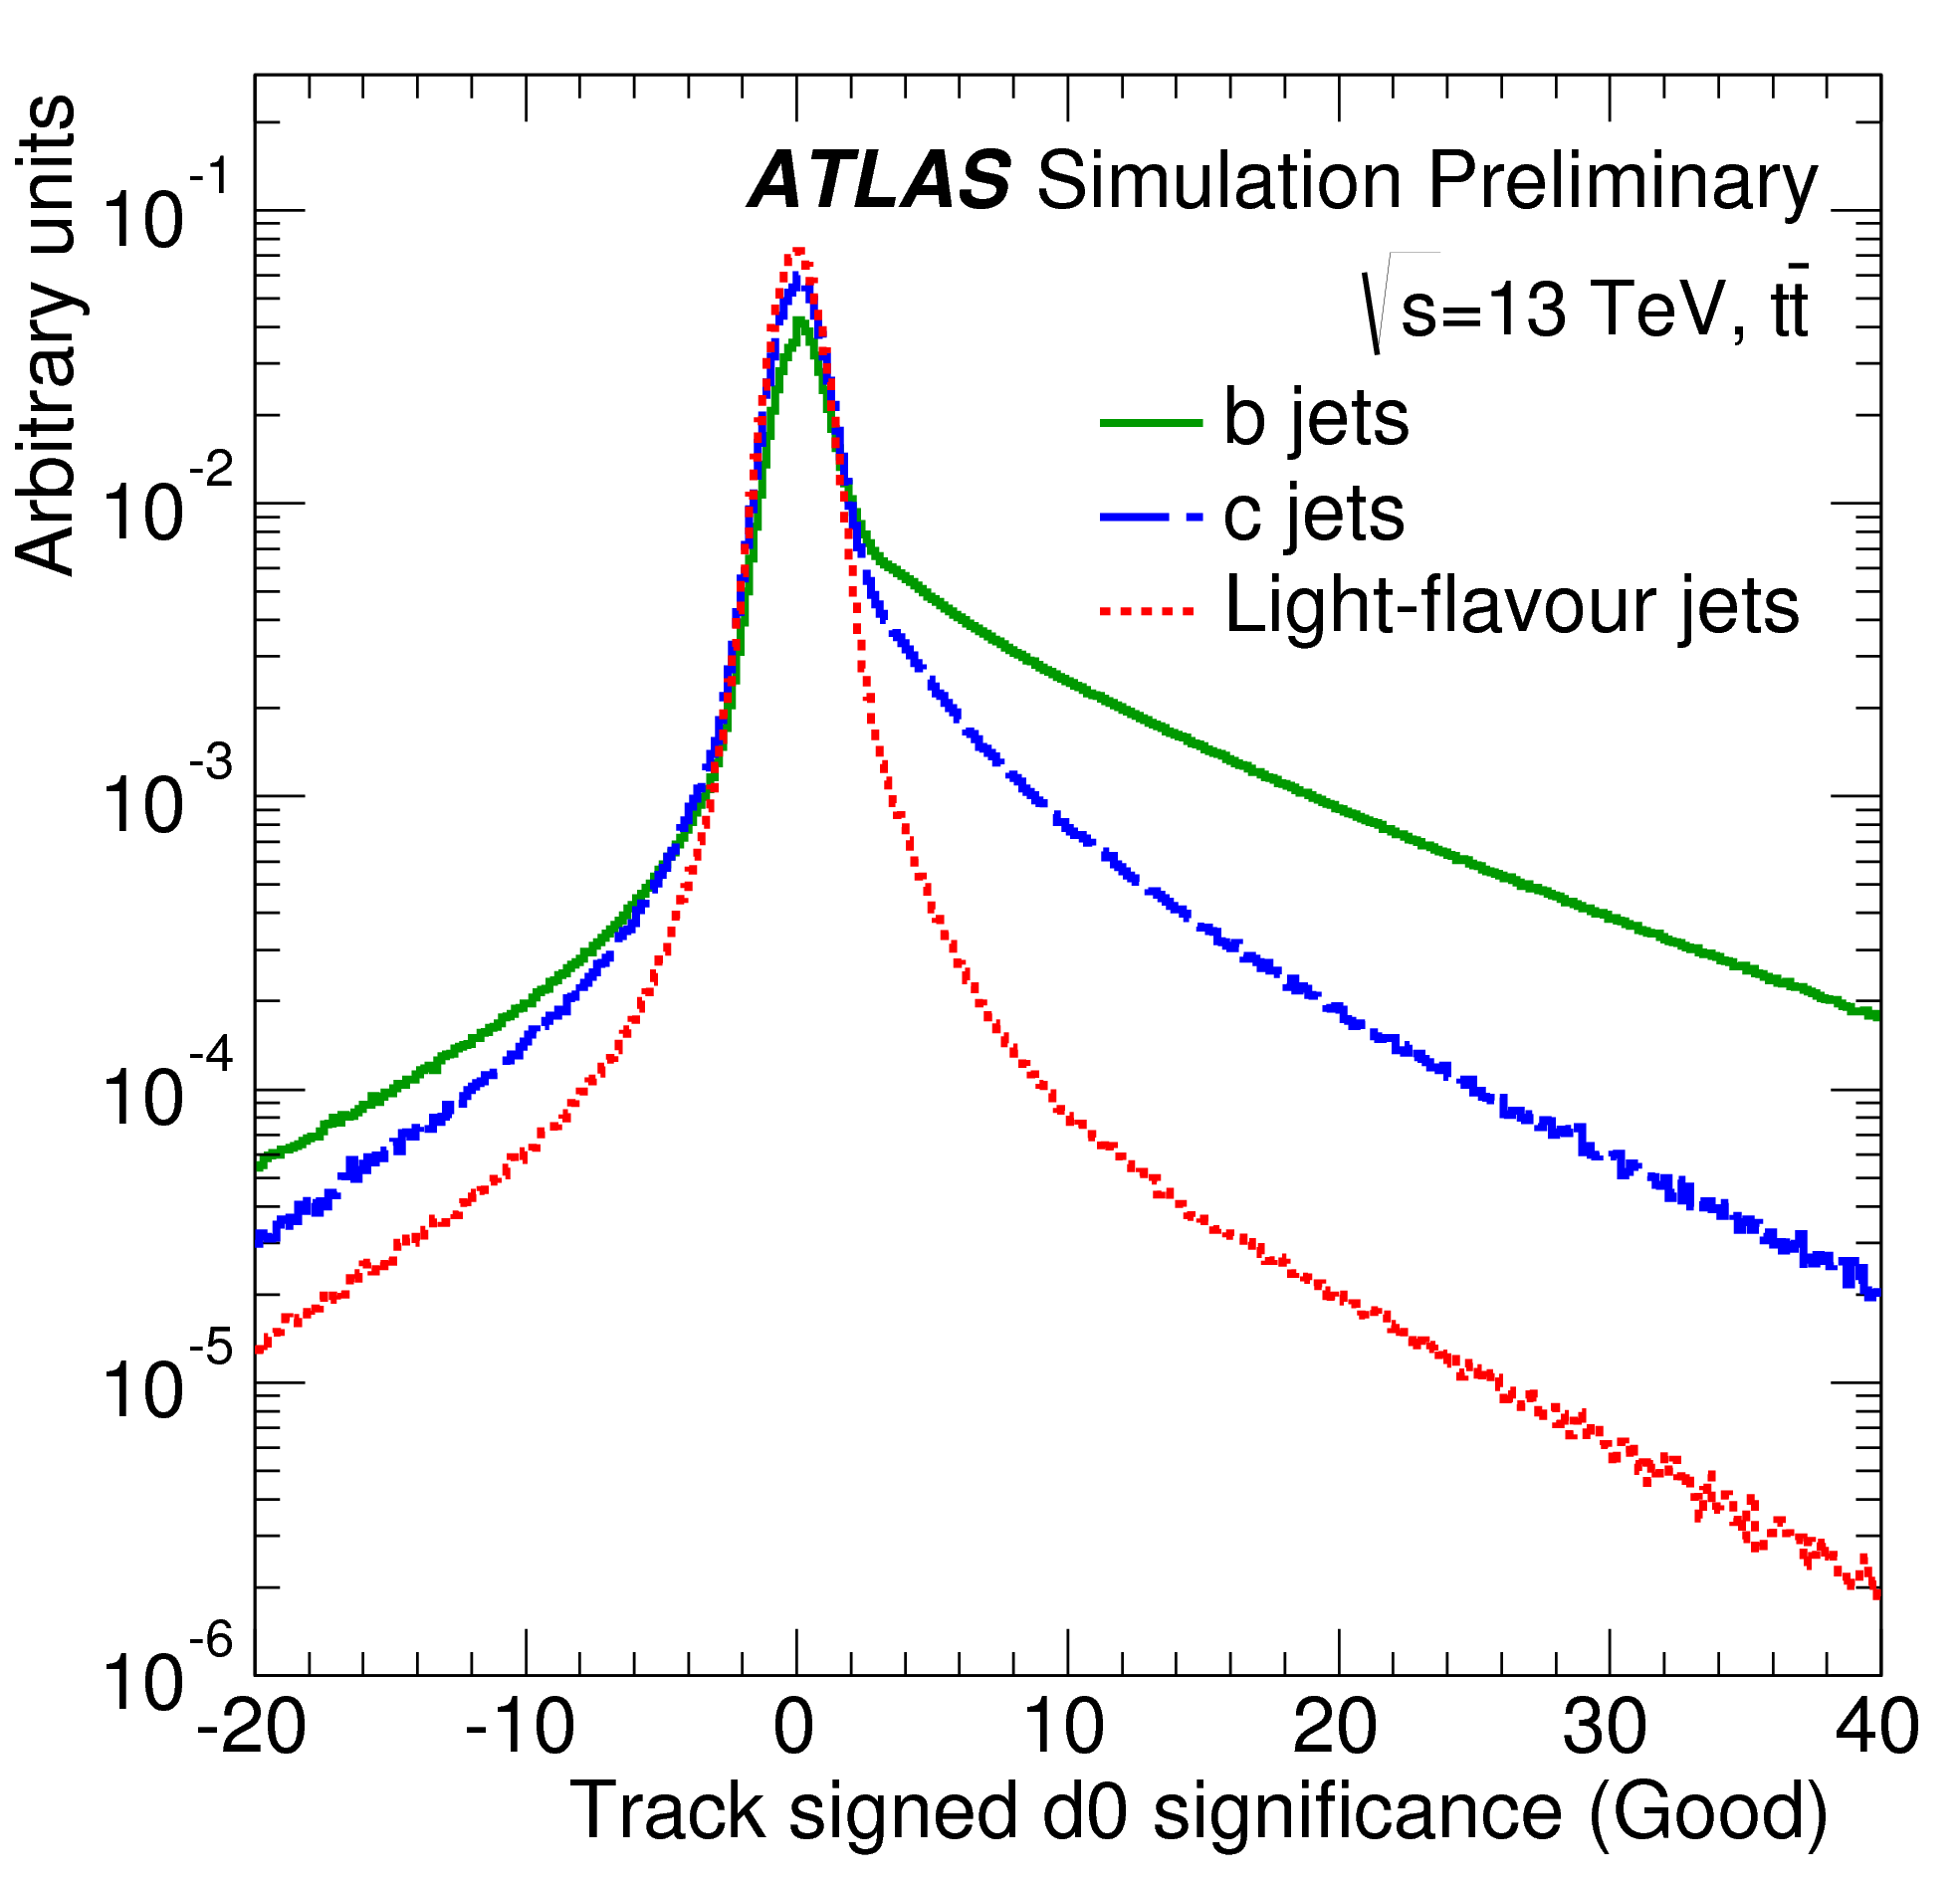
\includegraphics[width=0.49\textwidth]{Images/b-tagging/d0sig.png}}
\subfloat[]{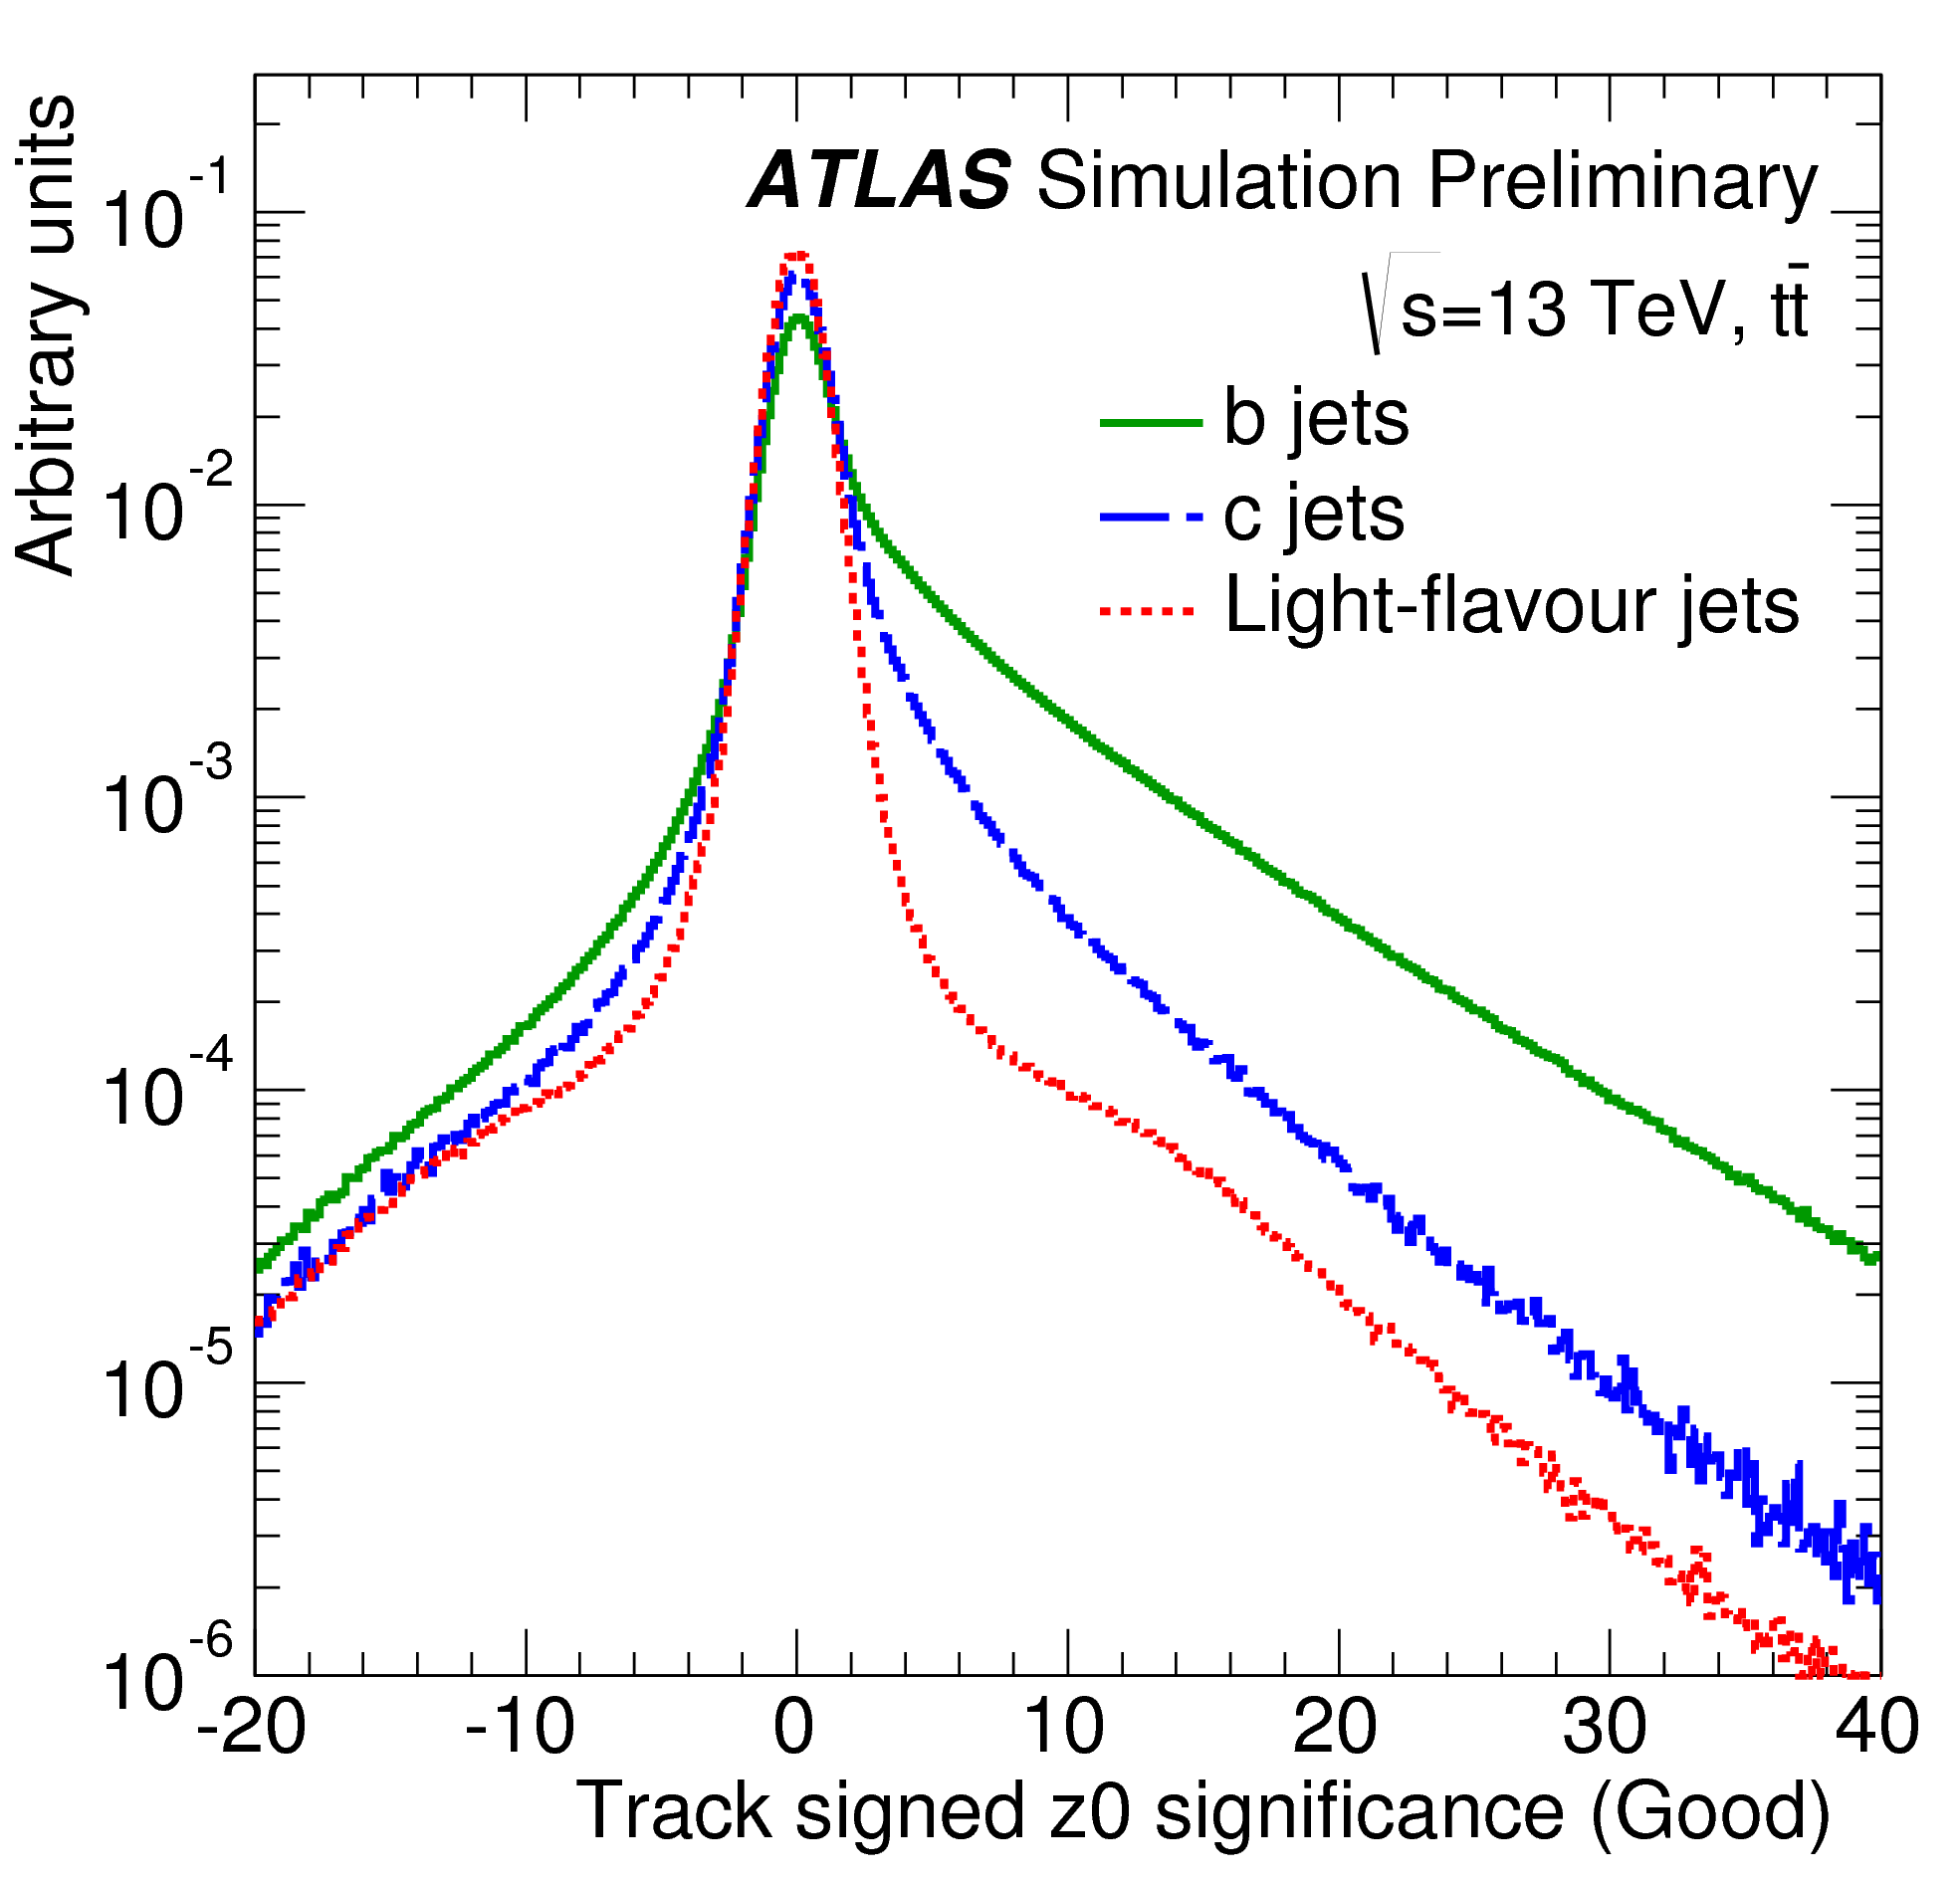
\includegraphics[width=0.49\textwidth]{Images/b-tagging/z0sig.png}}
\caption{The transverse (a) and longitudinal (b) signed impact parameter significance of tracks in tanti-t events associated with b (solid green), c (dashed blue) and light-flavor (dotted red) jets for the "Good" category defined in Table \ref{tab:track_tab}.}
\label{pic:dz0sig}
\end{figure}
Figure \ref{pic:dz0sig} shows the transverse and longitudinal impact parameter distributions for tracks from b-, c- and light-flavor jets. In the distribution of transverse impact parameter significances for light-flavor jets a clear exponential tail at high positive values is seen, corresponding to tracks from $K_S$ or $\Lambda$ decays, from photon conversions and interactions in the detector material. In the case of the longitudinal impact parameter significance, an additional component is seen in the tail, symmetric around zero, corresponding to tracks from pileup.
\begin{figure}
\subfloat[]{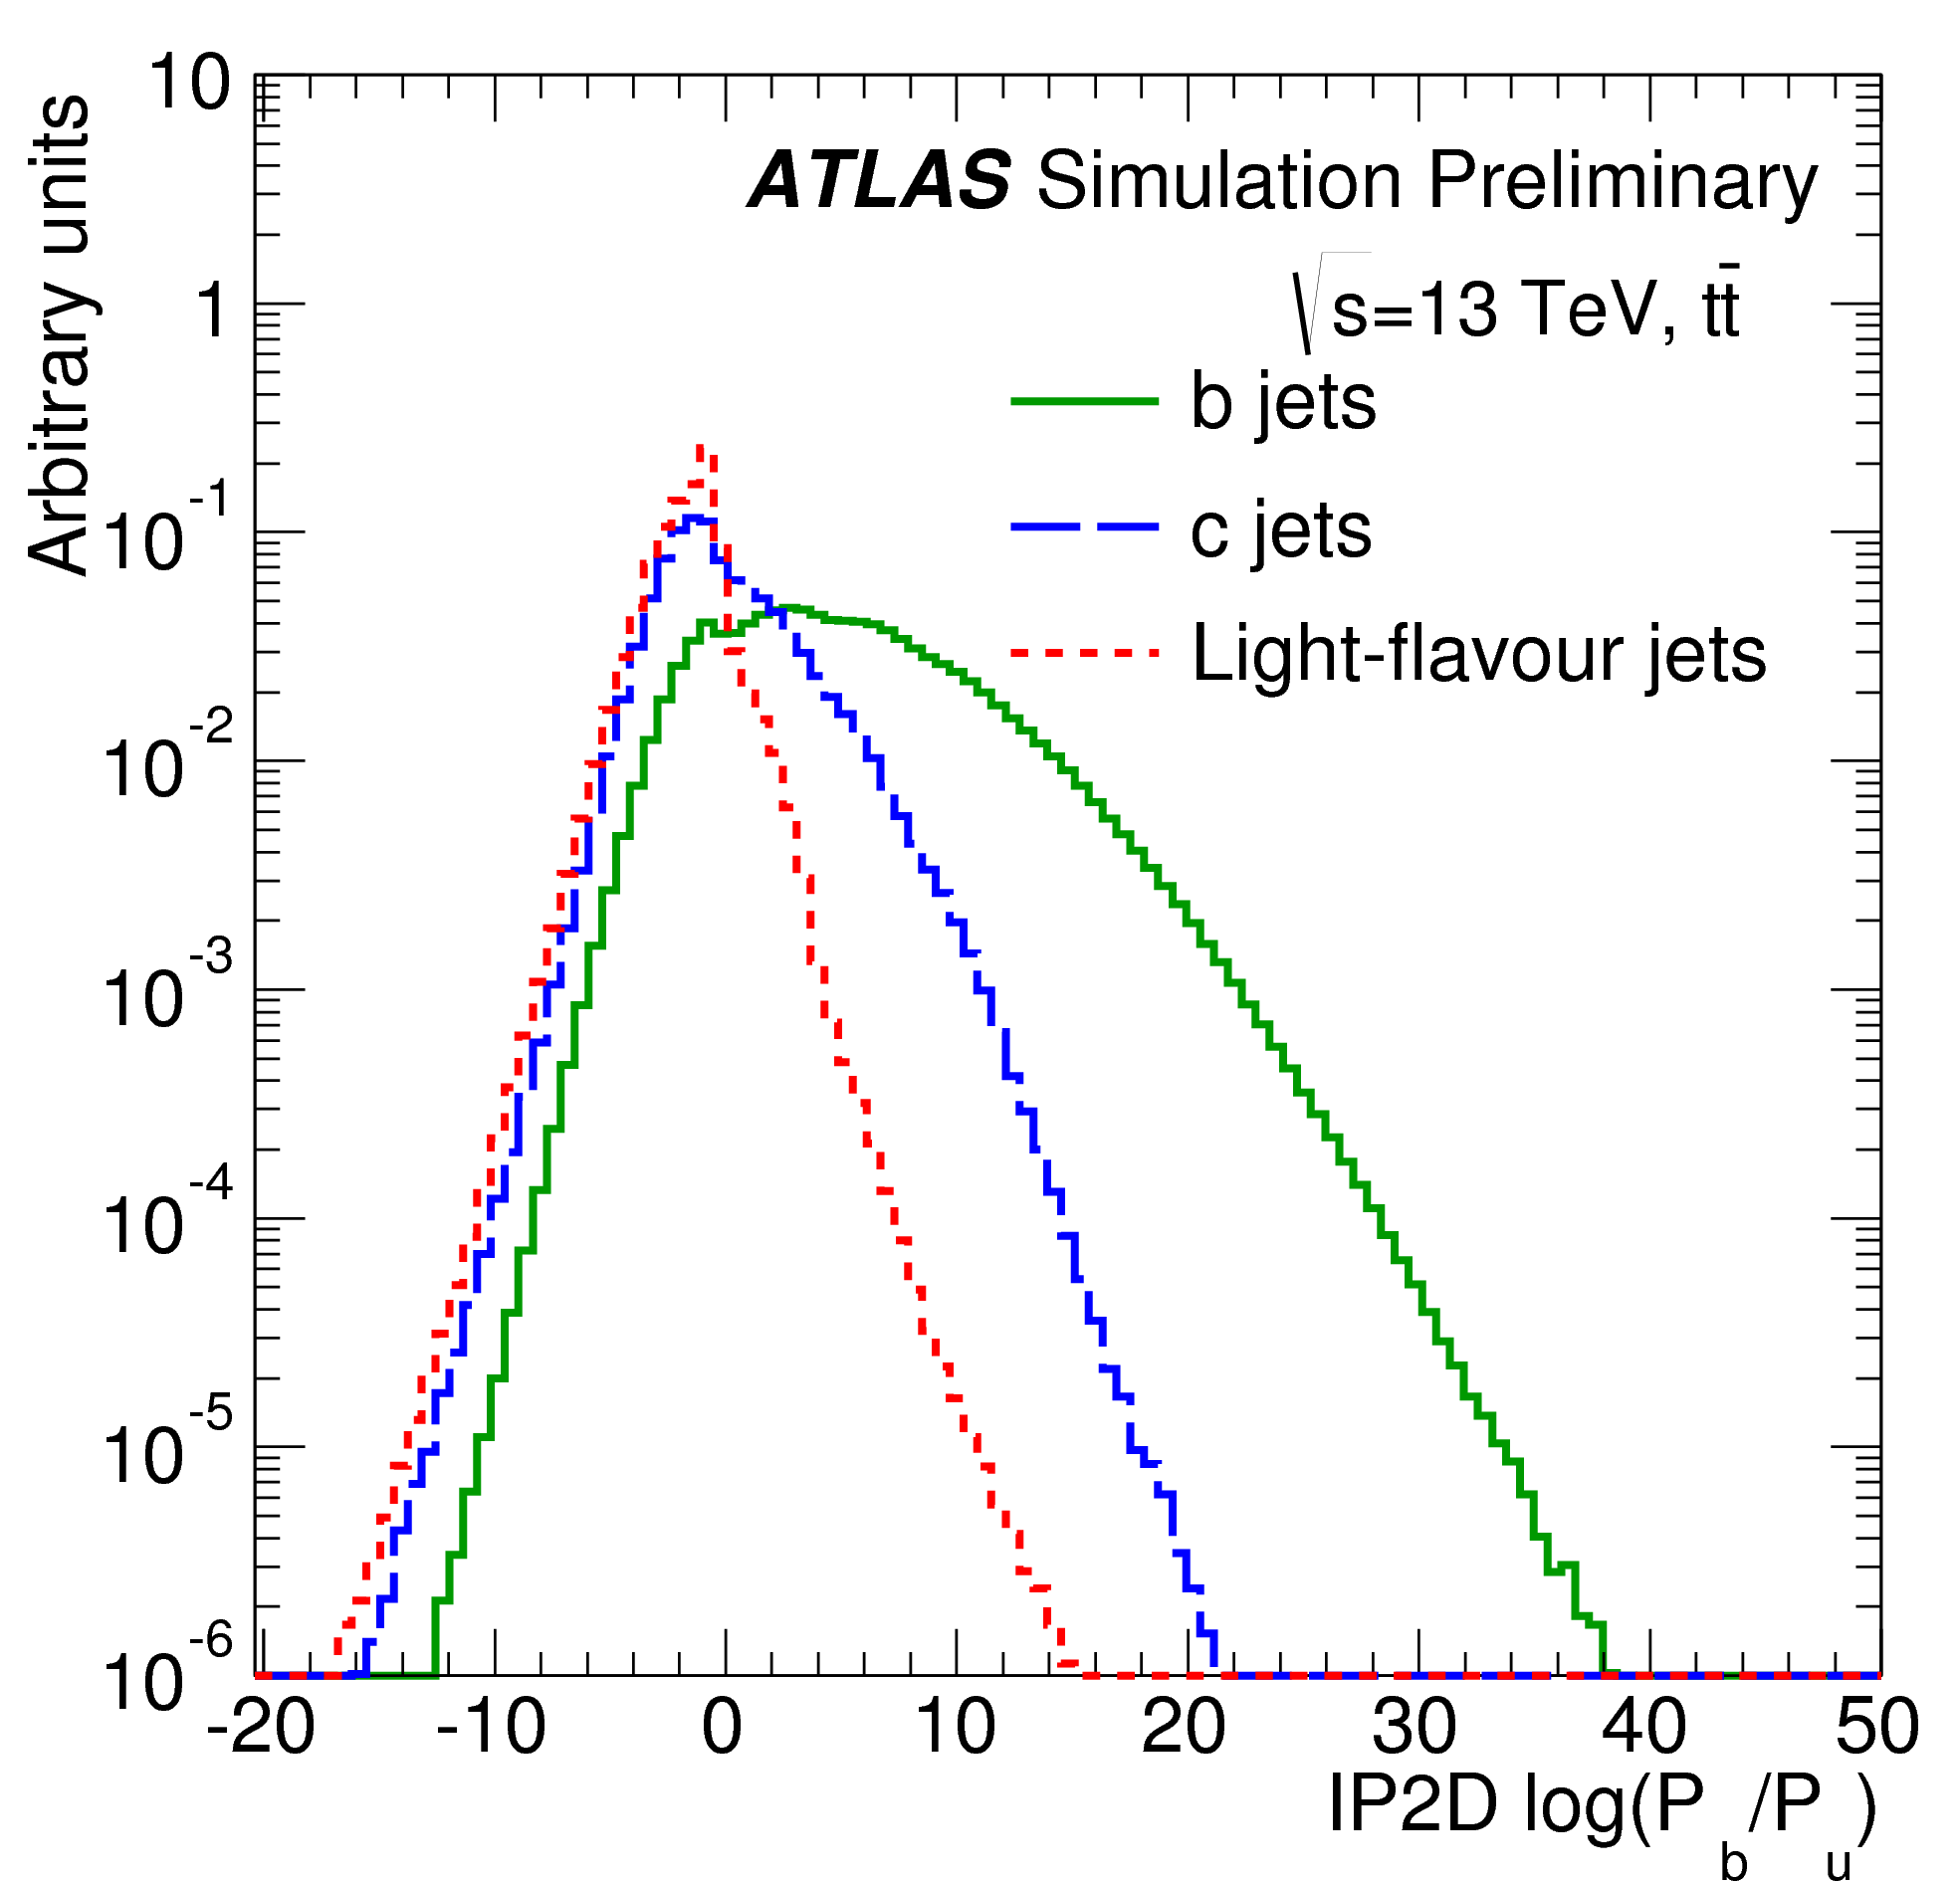
\includegraphics[width=0.49\textwidth]{Images/b-tagging/ip2d.png}}
\subfloat[]{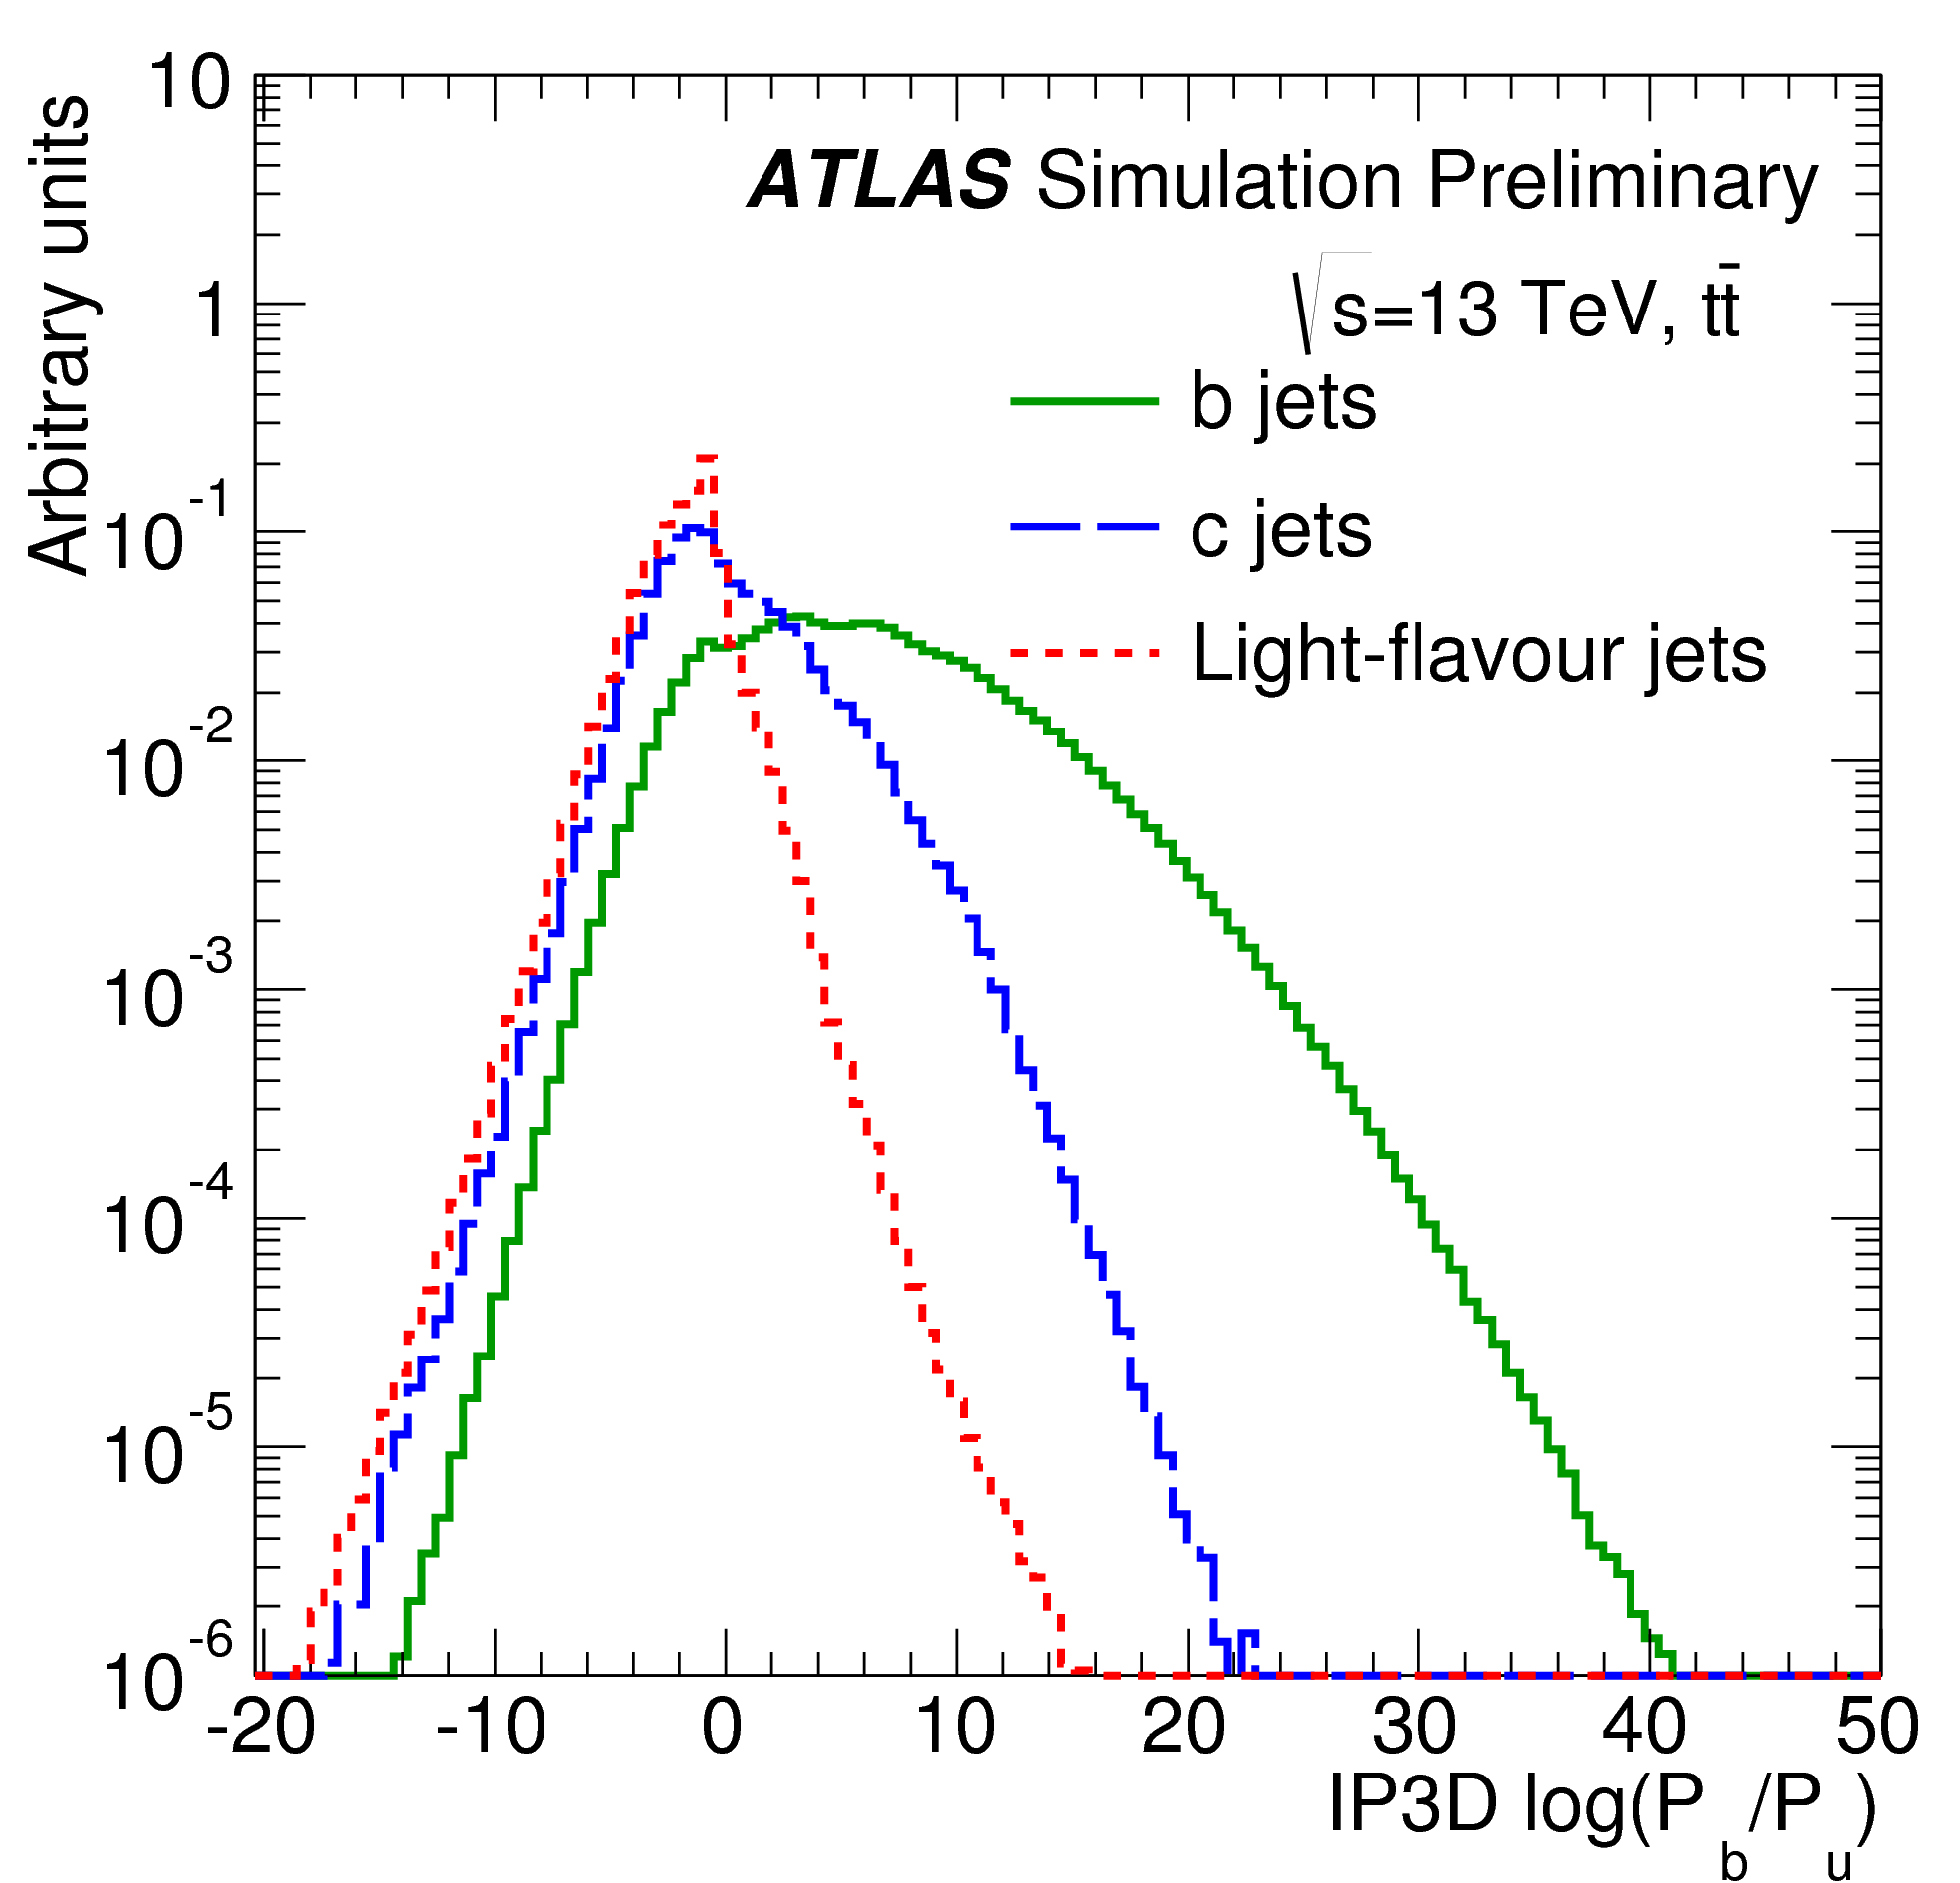
\includegraphics[width=0.49\textwidth]{Images/b-tagging/ip3d.png}}
\caption{The log likelihood ratio for the IP2D (a) and IP3D (b) b-tagging algorithm for b (solid green),
c (dashed blue) and light-flavor (dotted red) jets in $t \overline{t}$ events. If no tracks are found in the jet, a large
negative value is assigned as the algorithm output. This happens for less than 0.5\percent of b and c-jets, and
for about 2\percent of light-flavor jets.}
\label{pic:ipxd}
\end{figure}
The final discriminants for both the IP2D and IP3D algorithms are illustrated in Figure~\ref{pic:ipxd}

\subsubsection{Secondary vertex reconstruction in b-jets}
The explicit reconstruction of secondary vertex in b-jets can significantly improve the b-tagging performance of the impact parameter based algorithms. An exclusive reconstruction of the different possible b-decay modes cannot be performed with high efficiency: many od these decays modes involve neutral particles, which are difficult to reconstruct, and the set of selection cuts needed to reconstruct all the different decay modes would severely limit the reconstruction efficiency. The reconstruction of secondary b and c-hadron decay vertices in jets thus has to be done in an inclusive way, where the number of charged particle tracks originating from b and c hadron decay is not known a-priori.\\
Trying to resolve the b and c hadron vertices of the decay cascade is challenging for the following reasons:
\begin{itemize}
\item The probability to have at least two reconstructed charged particle tracks both from the b and c hadron decay is limited. This is due to the small charged particle multiplicities involved in this decay,  to the fact that some of the particle coming from b and c-hadron decay are compatible with the primary vertex and to the limited rack reconstruction efficiency.
\item The resolution of the relevant track parameters, especially at low transverse momenta, are not sufficient to separate the two vertices efficiently.
\end{itemize}
Two strategy to detect a secondary vertex in b-jets are available in ATLAS. The first one is based on a fit of single geometrical vertex. Even if this is not correct, this approximation works well for a large fraction of cases. The second algorithm is based on a kinematic approach, which assumes that the primary event vertex, the b-vertex and the c-vertex lie approximately on the same line, the flight path of the b-hadron.

\subsubsection{The secondary vertex finding algorithm: SV}
%The secondary vertex based algorithm \cite{BTAG_15} aims to explicitly reconstruct an inclusive displaced secondary
%vertex within the jet. The first step consists of reconstructing two-track vertices using the
%candidate tracks. Tracks are rejected if they form a secondary vertex which can be identified as likely
%originating from the decay of a long-lived particle (e.g. KS or ), photon conversions or hadronic
%interactions with the detector material. A single vertex is then reconstructed using the tracks that survive
%this preselection, with outlier tracks iteratively removed.
%\begin{figure}
%\subfloat[]{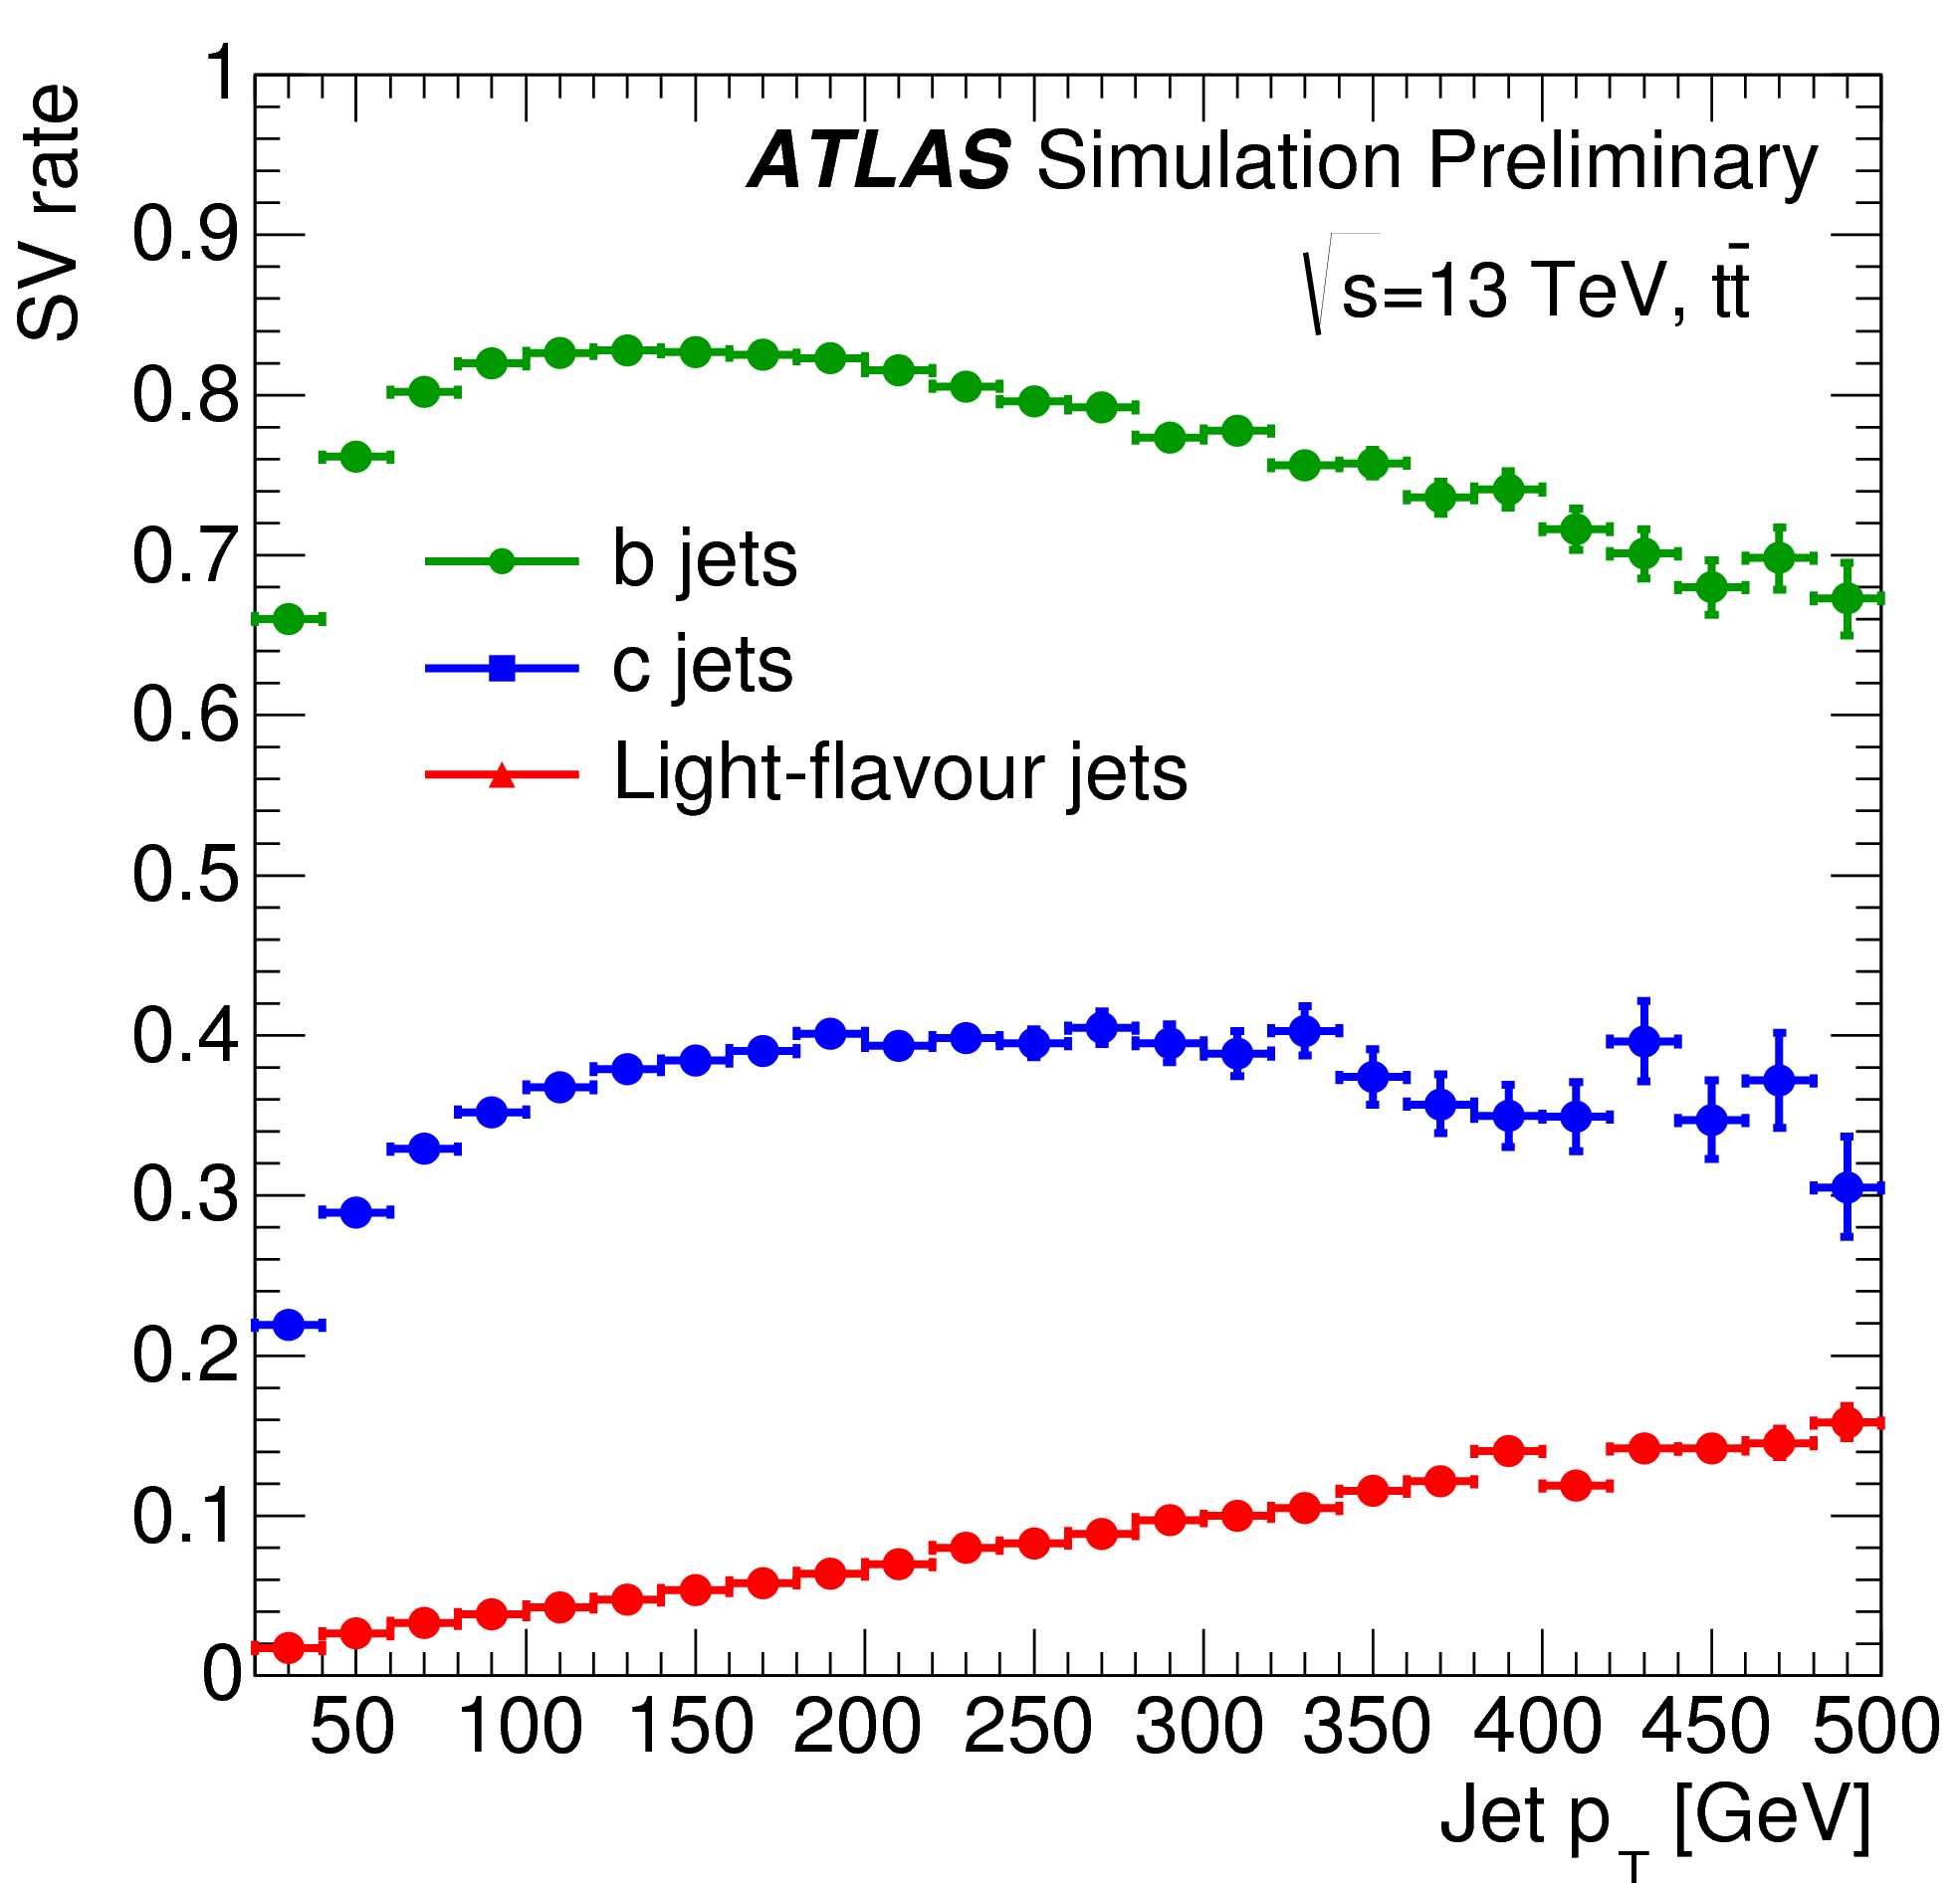
\includegraphics[width=0.49\textwidth]{Images/b-tagging/svrate_jetpt.png}}
%\subfloat[]{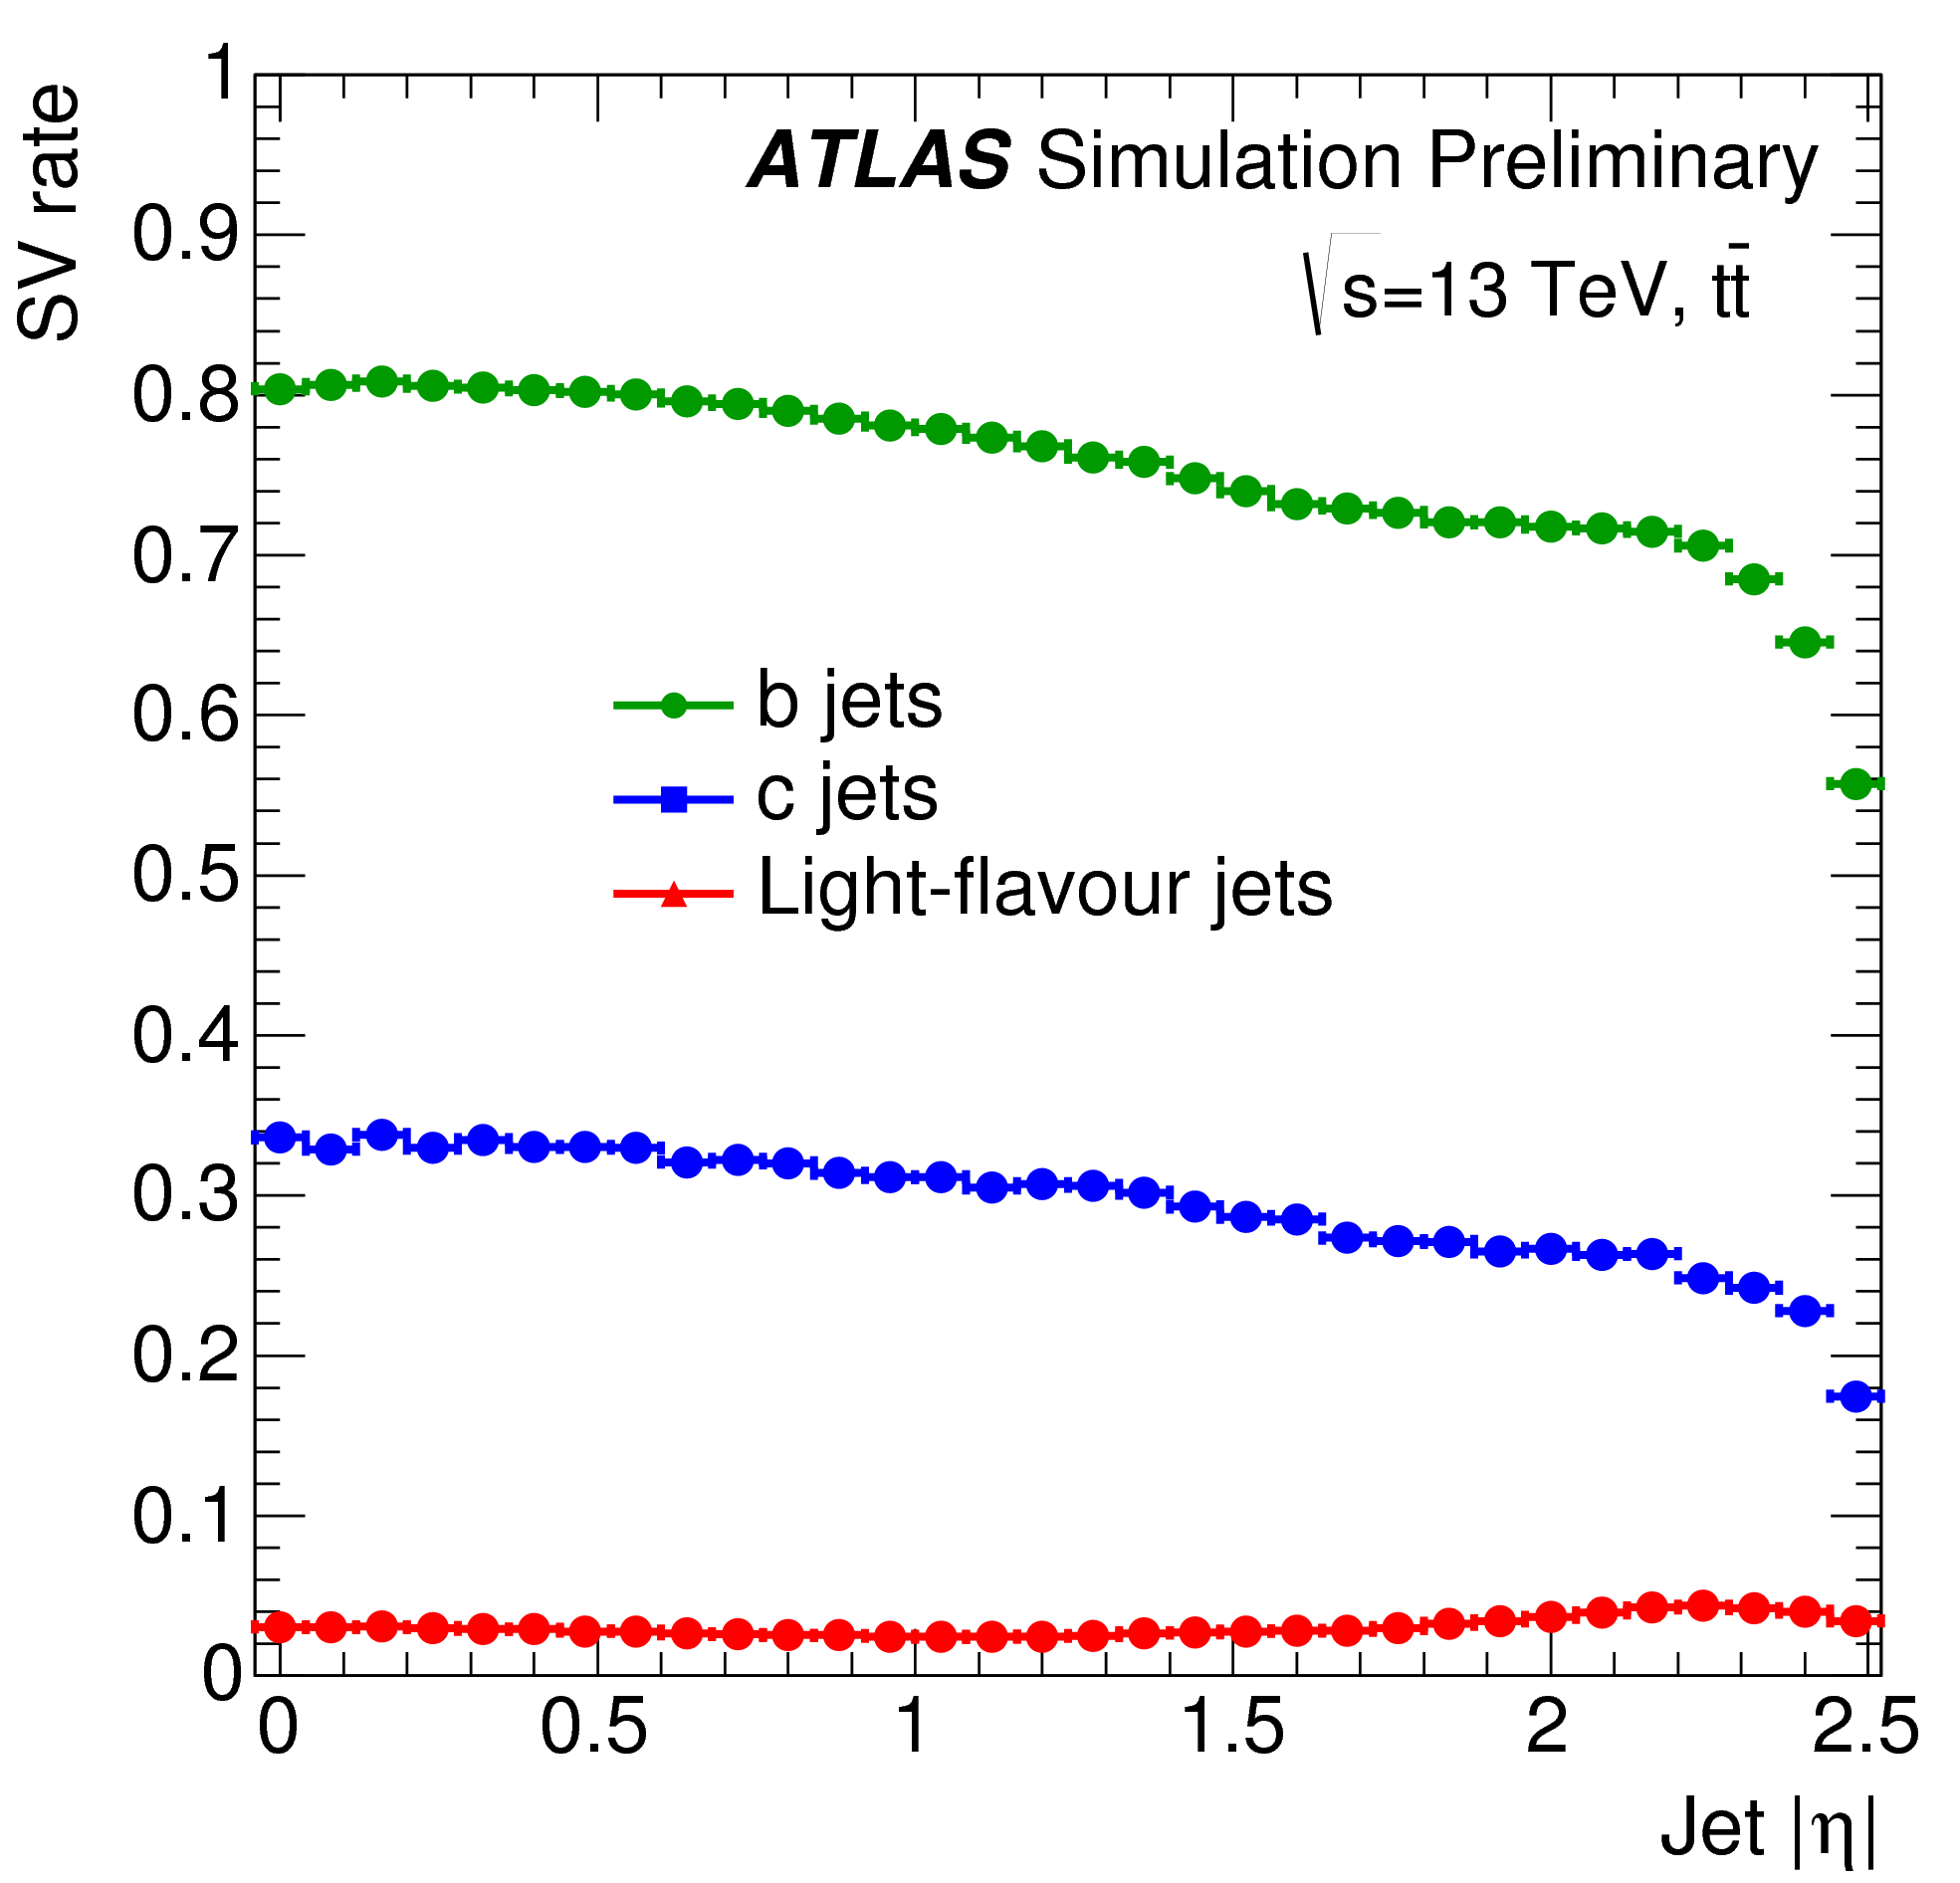
\includegraphics[width=0.49\textwidth]{Images/b-tagging/svrate_eta.png}}
%\caption{Secondary vertex reconstruction rate as function of jet pT (a) and ? (b) for b (green), c (blue) and light-flavor (red) jets in tanti-t events.}
%\label{pic:svrate}
%\end{figure}
%Figure \ref{fig:sv_rate} shows the secondary vertex
%reconstruction efficiency as function of jet pT and  for b-, c- and light-flavor jets. Figure 5 shows the
%distribution of some of the properties of the reconstructed secondary vertex comparing vertices from b,
%c and light-flavor jets.

\subsubsection{The JetFitter algorithm}
Jet Fitter is an inclusive secondary vertex reconstruction algorithm which exploits the topological structure of weak b an c-hadron decays inside a jet.
Differently to the SVF algorithm, described in the previous section, the JetFitter assumes that b and c-hadron decay on the same line defined through the b-hadron flight path. All charged particle tracks stemming from either the b and c-hadron decay thus intersect this b-hadron flight axis. There are several advantages to this method:
\begin{itemize}
\item Incomplete topologies can also be reconstructed (in principle even the topology with a single track from the b-hadron decay and a single track from the c-hadron decay is accessible).
\item The fit evaluates the compatibility if the given set of tracks with a b-c hadron like cascade topology, increasing the discrimination power against light quark jets.
\item Constraining the tracks to lie on the b-hadron flight axis reduces the degrees of freedom of the fit, increasing the chance to separate the b/c-hadron vertices. 
\end{itemize}
From the physics point of view this hypothesis is justified through the kinematics of the particles involved as defined through the hard b-quark fragmentation function and the masses of the b and c-hadrons. The lateral displacement of the c-hadron decay vertex with respect to the b-hadron flight path is small enough not to violate significantly the basic assumption within the typical resolutions of tracking detectors.
In JetFitter the vertexing task is mathematically implemented as an extension of the Kalman Filter (Section~\ref{sec:kalman_filter}) formalism for the vertex reconstruction. While a conventional Kalman Filter iteratively update the vertex position variables $\vv{x}$, the JetFitter algorithm is described through the following variables:
\begin{equation}
\vv{d} = (x_{PV},y_{PV},z_{PV},\phi,\theta,d_1, d_2, d_3,...,d_N)
\end{equation}
with:
\begin{itemize}
\item $(x_{PV},y_{PV},z_{PV})$: the primary vertex coordinates;
\item $(\phi,\theta)$: the azimuthal and the polar directions of the b-hadron flight axis;
\item $(d_1,...d_N)$: the distances of the fitted vertices, defined as the intersections of one or more tracks and the b-hadron flight axis, to the primary vertex position along the flight axis (N representing the number of vertices).
\end{itemize}
Before starting the fit, the variables are initialized with the information of the primary vertex position, provided by the primary vertex finding algorithm, and the b-hadron flight direction, approximated by the direction of the jet axis.
After this initialization a first fit is performed under the hypothesis that each track represents a single vertex along the b-hadron flight axis, until $\chi^2$ converged is reached, obtaining a first set of fitted $(\phi,\theta,d_1, d_2, d_3,...,d_N)$.
A clustering procedure is then performed, where all the combinations of two vertices (picked among the vertices lying on the b-hadron flight axis plus the primary vertex) are taken into consideration, using the vertex probability estimation techniques, described in details in \cite[Giacinto]. The vertex probability estimation technique provides the probability of a certain vertex to be compatible with the fitted decay chain and the probability for two initially separate vertices along the flight axis to be compatible with a single vertex and with the overall new resulting decay chain.
The vertices with the highest compatibility are merged, a new complete fit is performed with the new decay chain structure. This procedure is then iterated until no pairs of vertices with a probability above a certain threshold exist anymore. The result of this clustering procedure is a well defined decay chain topology with a certain association of tracks to vertices along the b-hadron flight axis, where each vertex possesses at least one track.
\subsubsection{Multivariate Algorithm: MV2}
\begin{figure}
\centering
\subfloat[]{\label{pic:mv2_skeleton}\includegraphics[width=0.5\textwidth]{Images/b-tagging/mv2_sheme.png}}
\subfloat[]{\label{tab:MV2_var}\includegraphics[width=0.5\textwidth]{Images/b-tagging/MV2.png}}
\caption{(a) MV2 SKELETON (b) The MV2c20 output for b- (solid green), c- (dashed blue) and light-flavor (dotted red) jets in tanti-t events.}
\end{figure}
The b-tagging final algorithm is called MV2 and it's a boosted decision tree that take as input the output of the algorithms previously described as shown in Figure~\ref{pic:mv2_skeleton}.
%Boosted decision trees have been successfully used in High Energy Physics analysis for example by the MiniBooNE experiment (Yang-Roe-Zhu, physics/0508045).
In Boosted Decision Trees, the
selection is done on a majority vote on the result of several decision
trees, which are all derived from the same training sample by
supplying different event weights during the training.
Successive decision nodes are used to categorize the
events out of the sample as either signal or background. Each node
uses only a single discriminating variable to decide if the event is
signal-like or background-like. 
%This forms a tree like structure with "baskets" at the end (leave nodes), and an event is classified as either signal or background according to whether the basket where it ends up has been classified signal or background during the training. Training of a decision tree is the process to define the "cut criteria" for each node.
The training starts with the root node. Here one takes the full training event
sample and selects the variable and corresponding cut value that gives
the best separation between signal and background at this stage. Using
this cut criterion, the sample is then divided into two subsamples, a
signal-like (right) and a background-like (left) sample. Two new nodes
are then created for each of the two sub-samples and they are
constructed using the same mechanism as described for the root
node. The devision is stopped once a certain node has reached either a
minimum number of events, or a minimum or maximum signal purity. These
leave nodes are then called "signal" or "background" if they contain
more signal respective background events from the training sample.
The idea behind adaptive boosting is, that signal events
from the training sample, that end up in a background node
(and vice versa) are given a larger weight than events that are in
the correct leave node. This results in a re-weighed training event
sample, with which then a new decision tree can be developed.
The boosting can be applied several times (typically 100-500 times)
and one ends up with a set of decision trees (a forest).
Gradient boosting works more like a function expansion approach, where
each tree corresponds to a summand. The parameters for each summand (tree)
are determined by the minimization of a error function (binomial log-
likelihood for classification and Huber loss for regression).
A greedy algorithm is used, which means, that only one tree is modified
at a time, while the other trees stay fixed.
The input variables obtained from the three basic algorithms are combined  to discriminate b-jets from light (u,d,s-quark or gluon jets) and c-jets. The training is
performed on a set of approximately 5 million $t\overline{t}$ events. The MV2c20 algorithm is defined as the output
of such a boosted decision three with the training performed assigning b-jets as signal and a mixture of 80\percent light-flavor
jets and 20\percent c-jets as background.
\begin{table}
\begin{center}
\begin{tabular}{|c|c|p{8cm}|}
\hline
Input & Variable & Description \\
\hline
Kinematics & \pt (jet)  & Jet transverse momentum \\
& $\eta$ (jet) & Jet pseudo-rapidity\\
\hline
IP2D, IP3D & log(Pb=Plight) & Likelihood ratio between the b- and light jet hypotheses \\
 & log(Pb=Pc ) & Likelihood ratio between the b- and c-jet hypotheses \\
 & log(Pc=Plight) & Likelihood ratio between the c- and light jet hypotheses \\
\hline
SV & m (SV) & Invariant mass of tracks at the secondary vertex assuming pion masses \\
& $f_E$(SV) & Fraction of the charged jet energy in the secondary vertex \\
 & NTrkAtVtx(SV) & Number of tracks used in the secondary vertex \\
 & N2TrkVtx (SV) & Number of two track vertex candidates \\
 & $L_{xy}$ (SV) & Transverse distance between the primary and secondary vertices \\
 & $L_{xyz}$ (SV) & Distance between the primary and secondary vertices \\
 & $S_{xyz}$ (SV) & Distance between the primary and secondary vertices divided by its uncertainty\\
 & R(jet;SV) & R between the jet axis and the direction of the secondary vertex relative to the primary vertex\\
\hline
Jet Fitter & N2TrkVtx (JF) & Number of 2-track vertex candidates (prior to decay chain fit) \\
 & m(JF) & Invariant mass of tracks from displaced vertices assuming pion masses \\
 & $S_{xyz}$(JF) & Significance of the average distance between the primary and displaced vertices\\
 & $f_E$v(JF) &  Fraction of the charged jet\\
 \hline
\end{tabular}
\caption{The 24 input variables used by the MV2c00 and MV2c20 b-tagging algorithm.}
\labe{}
\end{center}
\end{table}
The list of input variables used for the training is summarized in
Table~\ref{tab:MV2_var}. The kinematic properties (\pt and $\eta$) of the jets are included in the training to take advantage
of correlations with the other input variables. In order to avoid any difference in the kinematic spectra
between signal and background jets being interpreted as discriminant by the training, the signal jets are
re-weighted to match the spectrum of the background jets.


The MV2c20 output distribution is shown in Figure~\ref{pic:mv2_out} for b, c and light-flavor jets.
\subsection{The b-tagging performance}
%It is of interest to determine the total improvement in the b-tagging performance achieved between Run- 1 and \runtwo due to the addition of the IBL and the algorithmic updates.
The \runtwo baseline algorithm for b-tagging was completely renewed during the long shutdown, and with the insertion of the IBL will improve the b-tagging performance. In Section~\ref{sec:btagperformance} the impact of the IBL on b-tagging performance have been showed. That study used a \runtwo based algorithm comparison.
\begin{figure}
\centering
\null\hfill
\subfloat[]{\label{pic:mv2_light}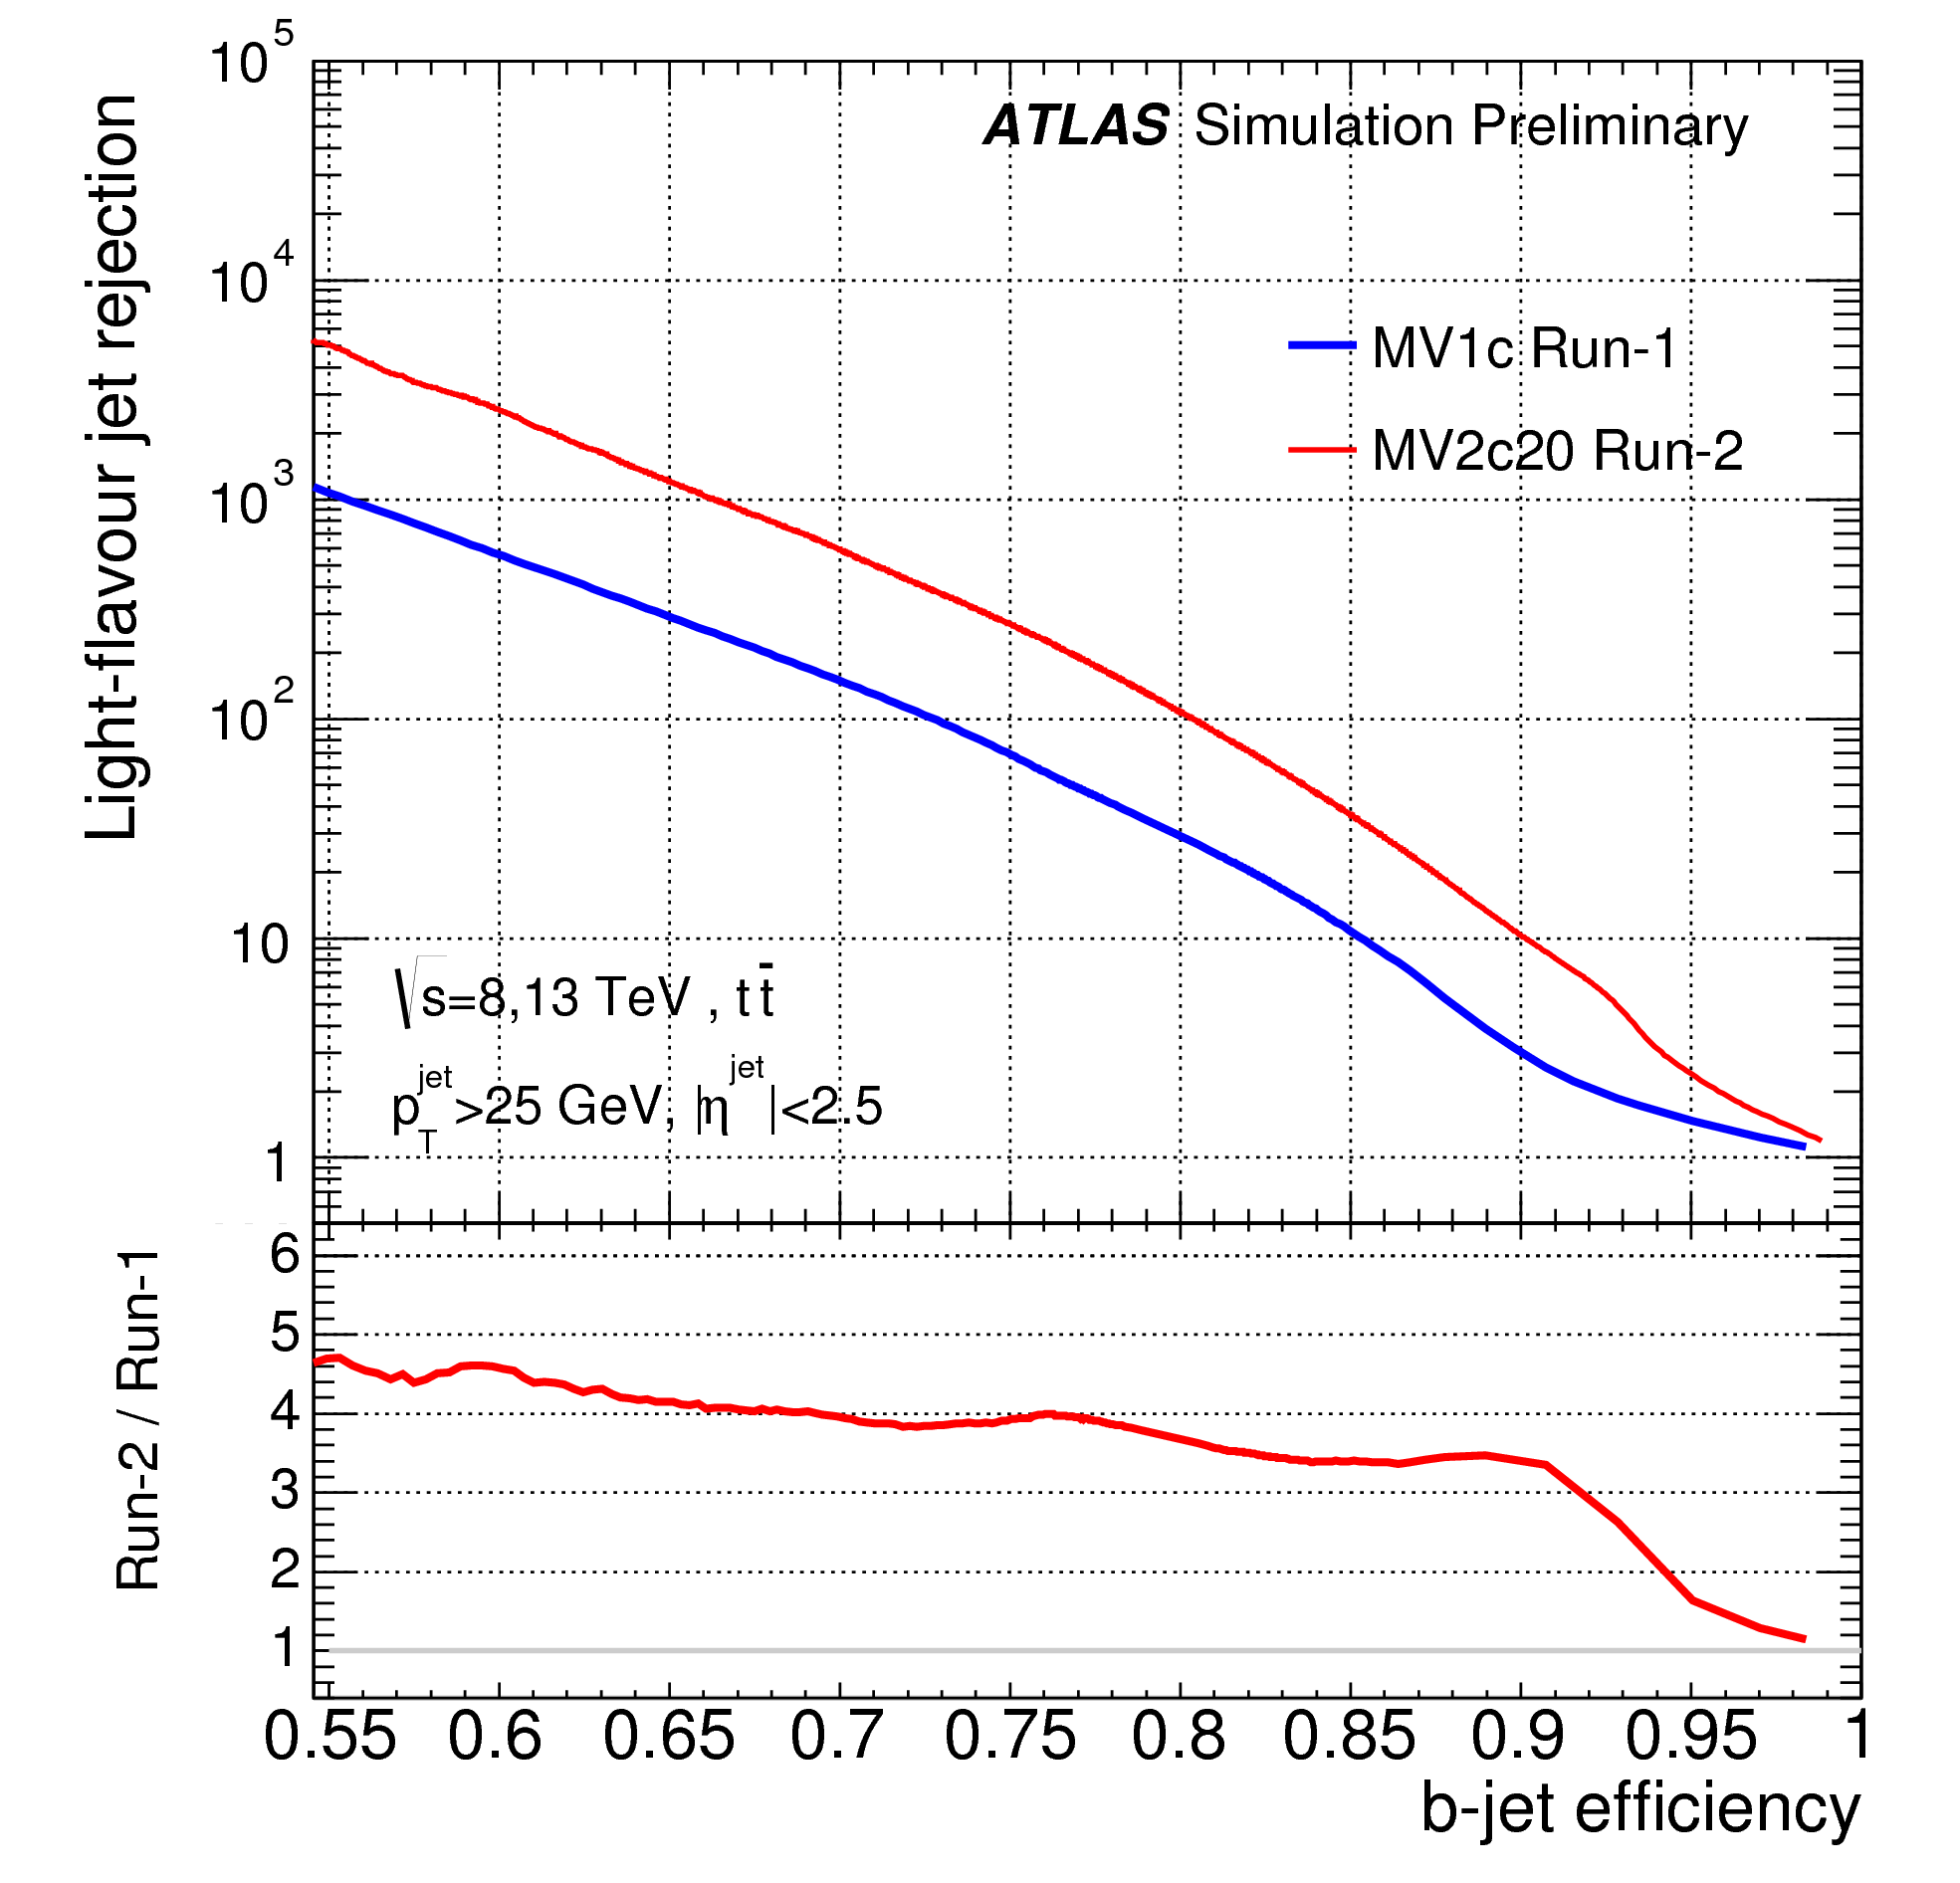
\includegraphics[width=0.5\textwidth]{Images/b-tagging/MV2vsMV1_lightrej.png}}
\hfill
\subfloat[]{\label{pic:mv2_c}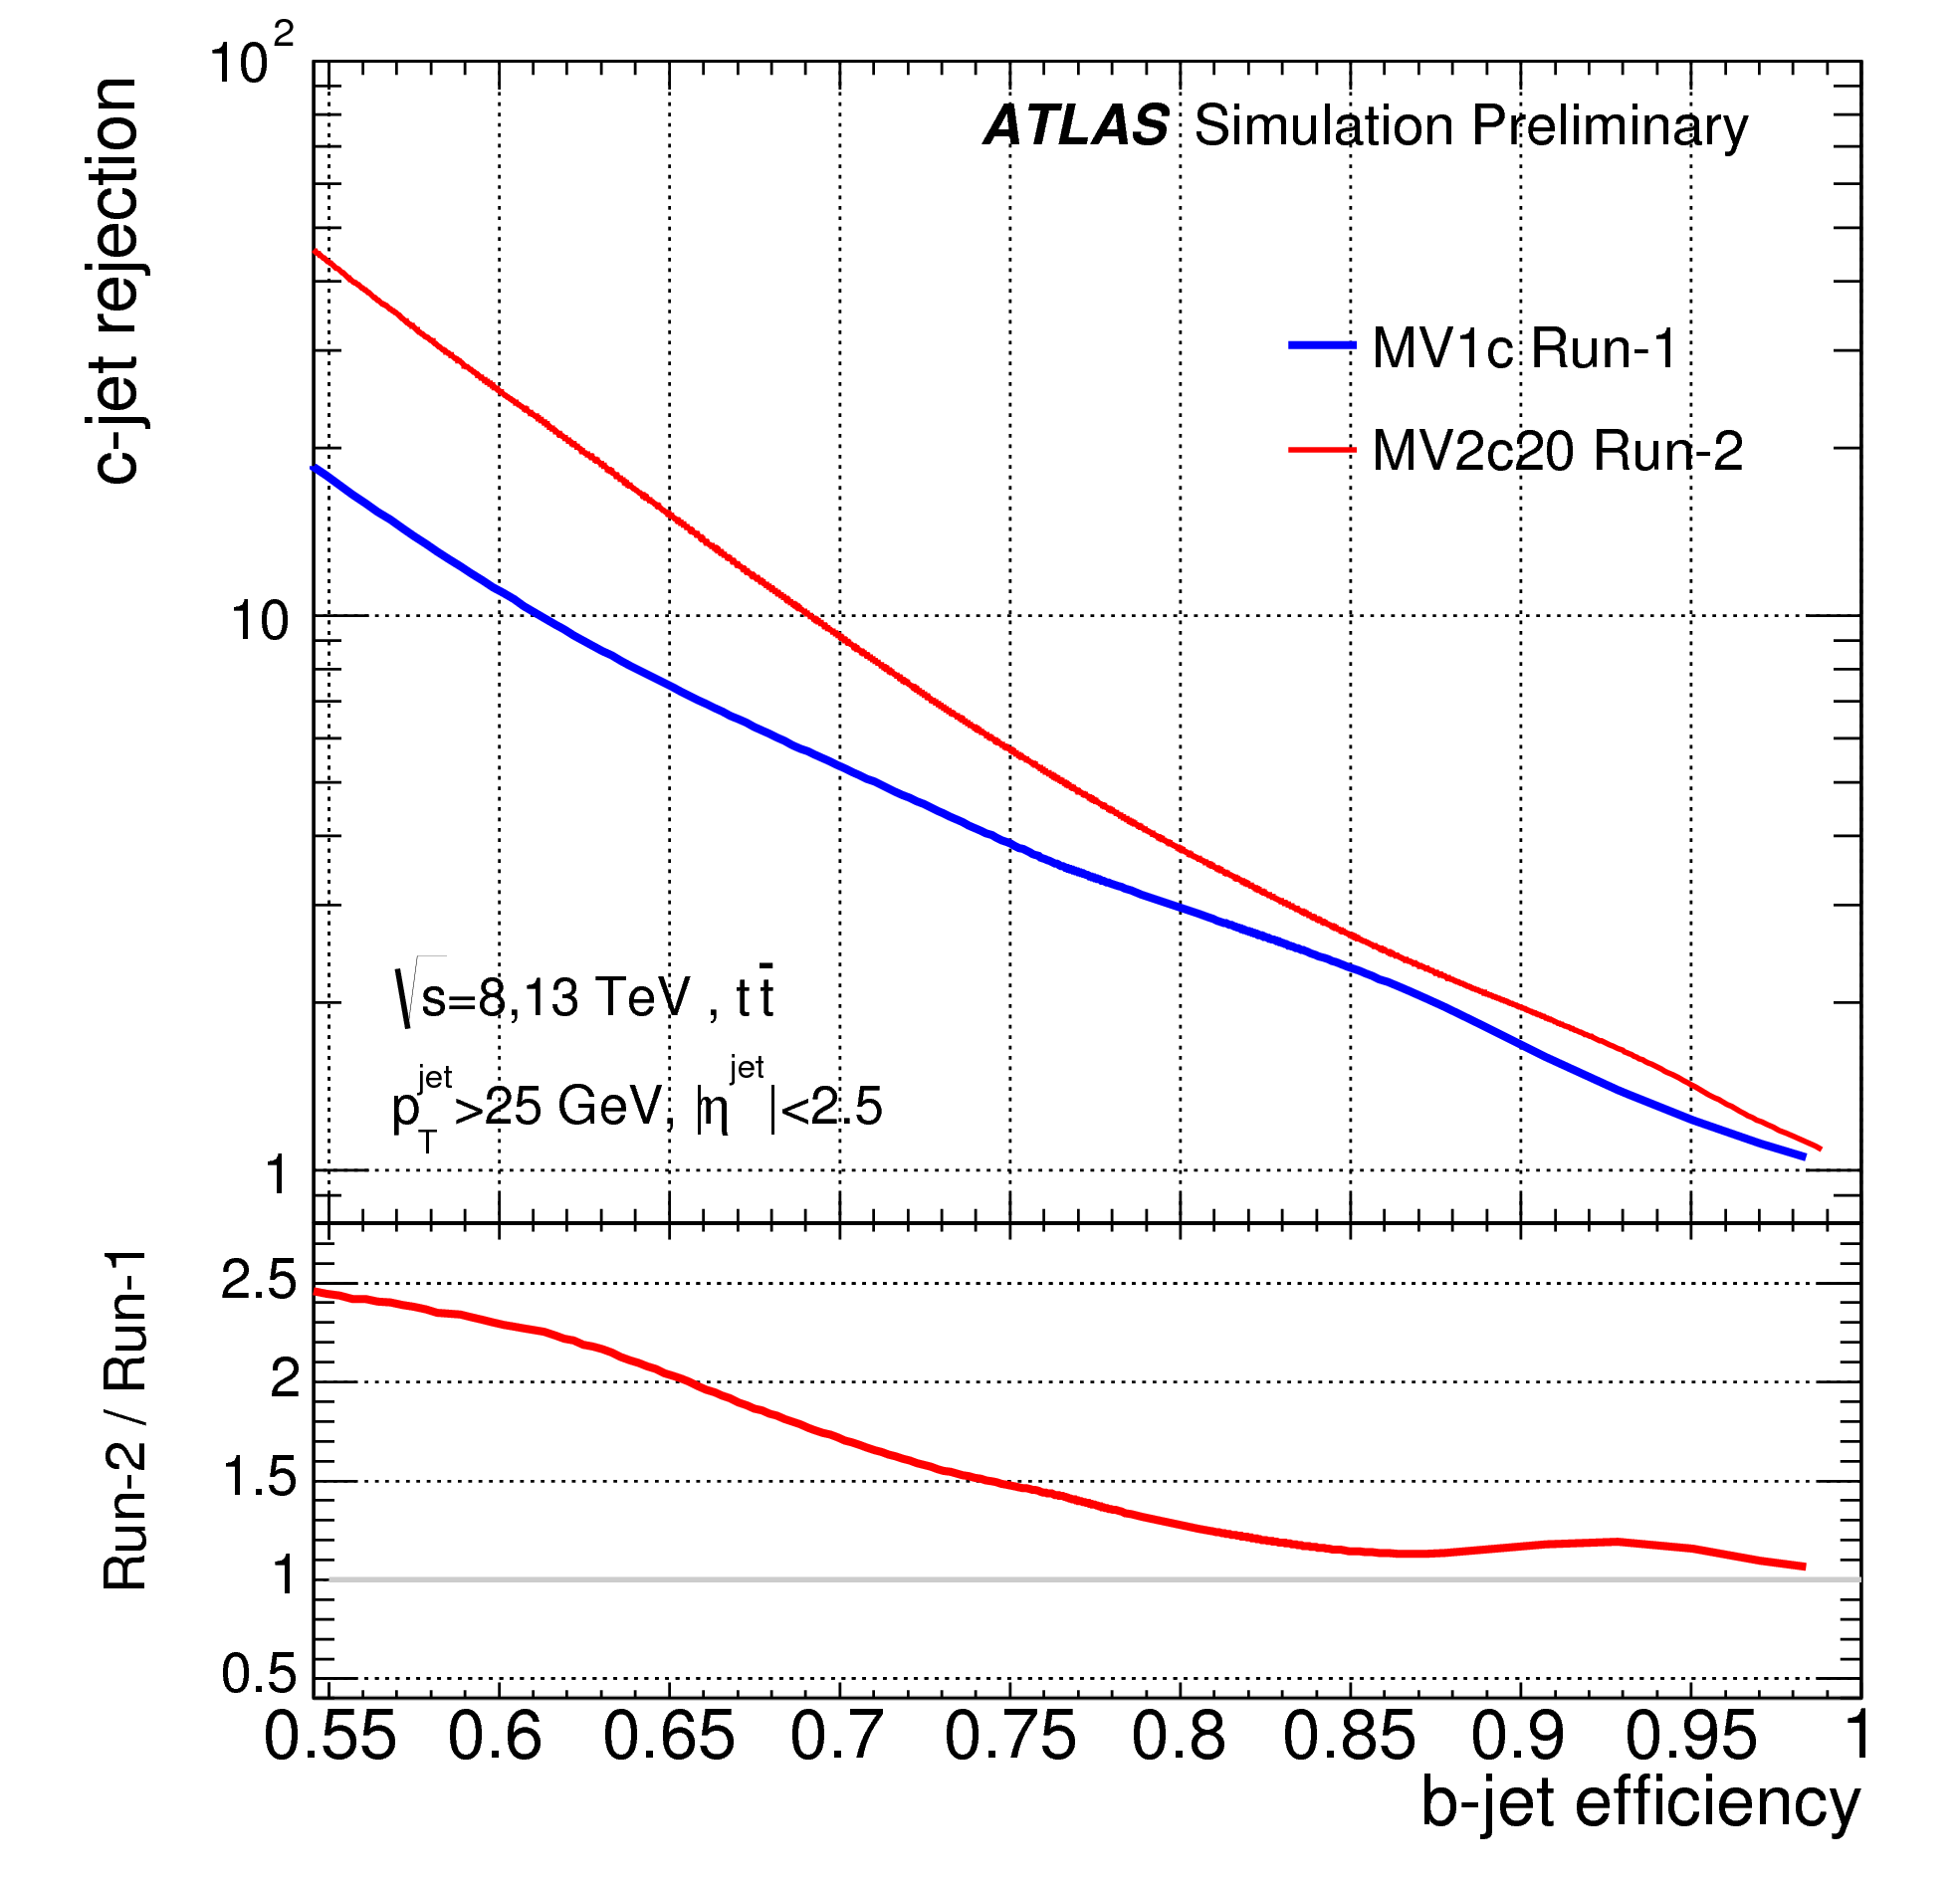
\includegraphics[width=0.5\textwidth]{Images/b-tagging/MV2vsMV1_crej.png}}
\hfill \null
\null \hfill
\subfloat[]{\label{pic:mv2_jetpt}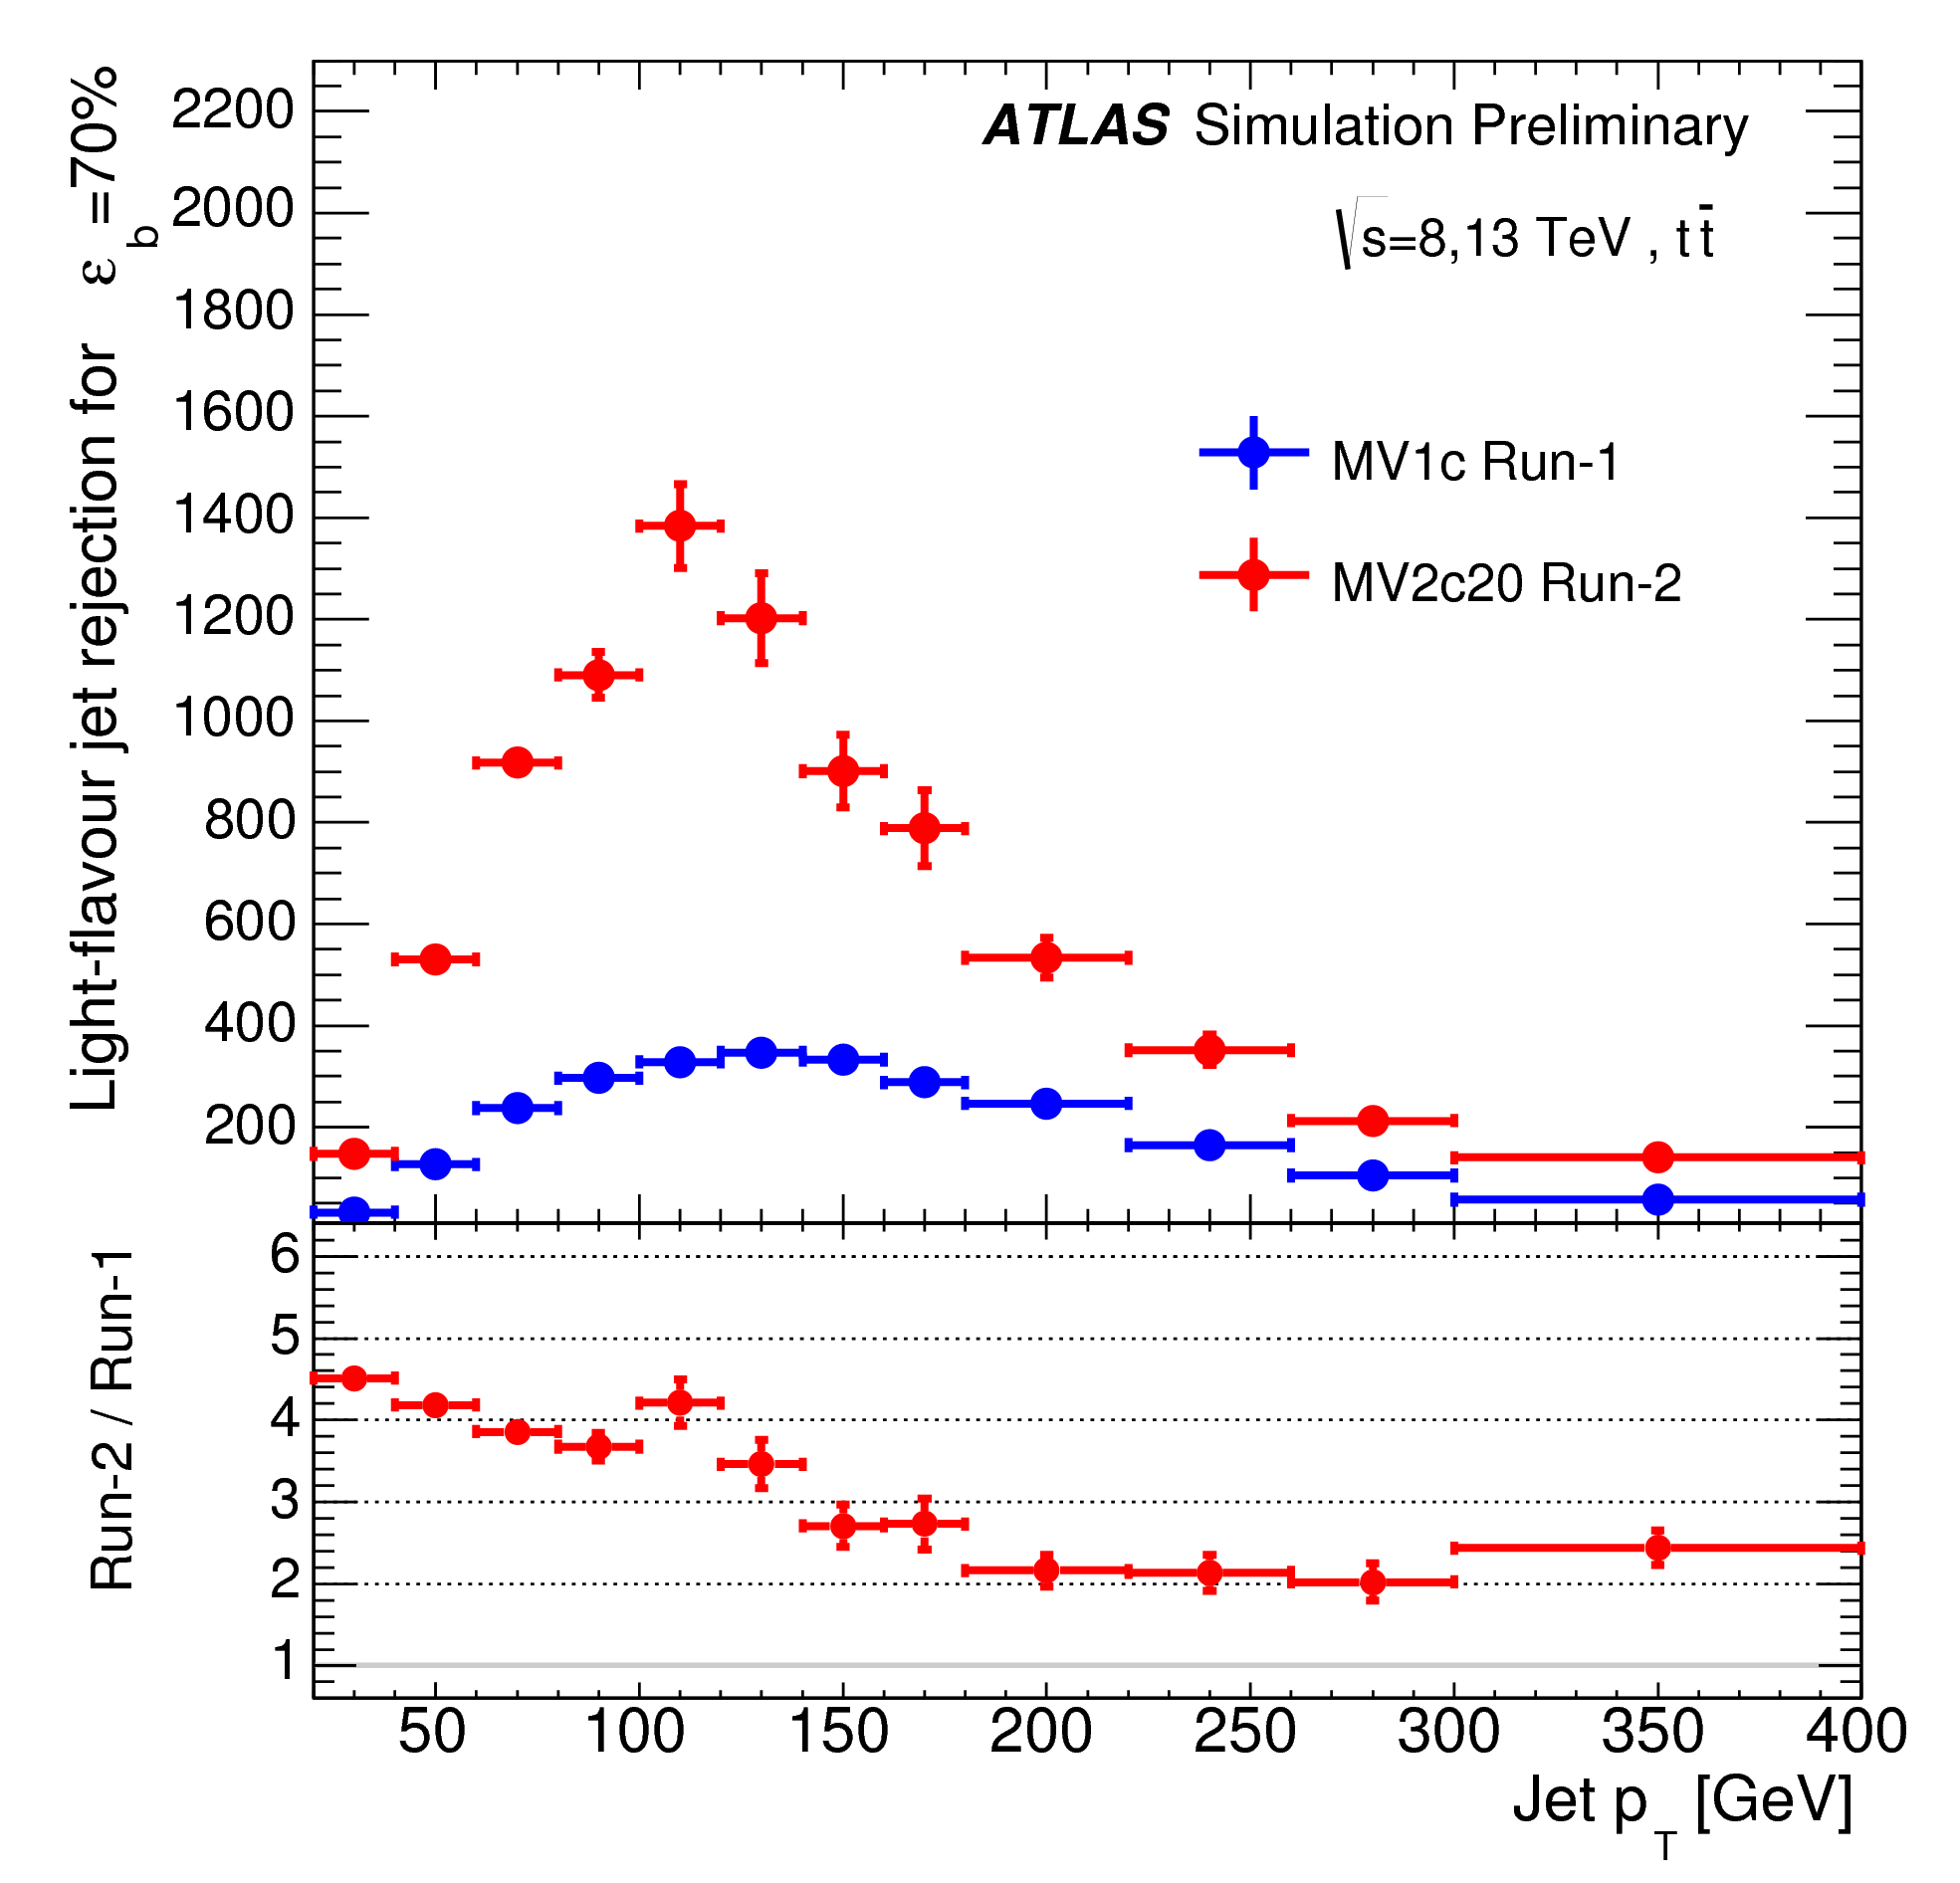
\includegraphics[width=0.5\textwidth]{Images/b-tagging/MV2vsMV1_jetpt.png}}
\hfill
\subfloat[]{\label{pic:mv2_eta}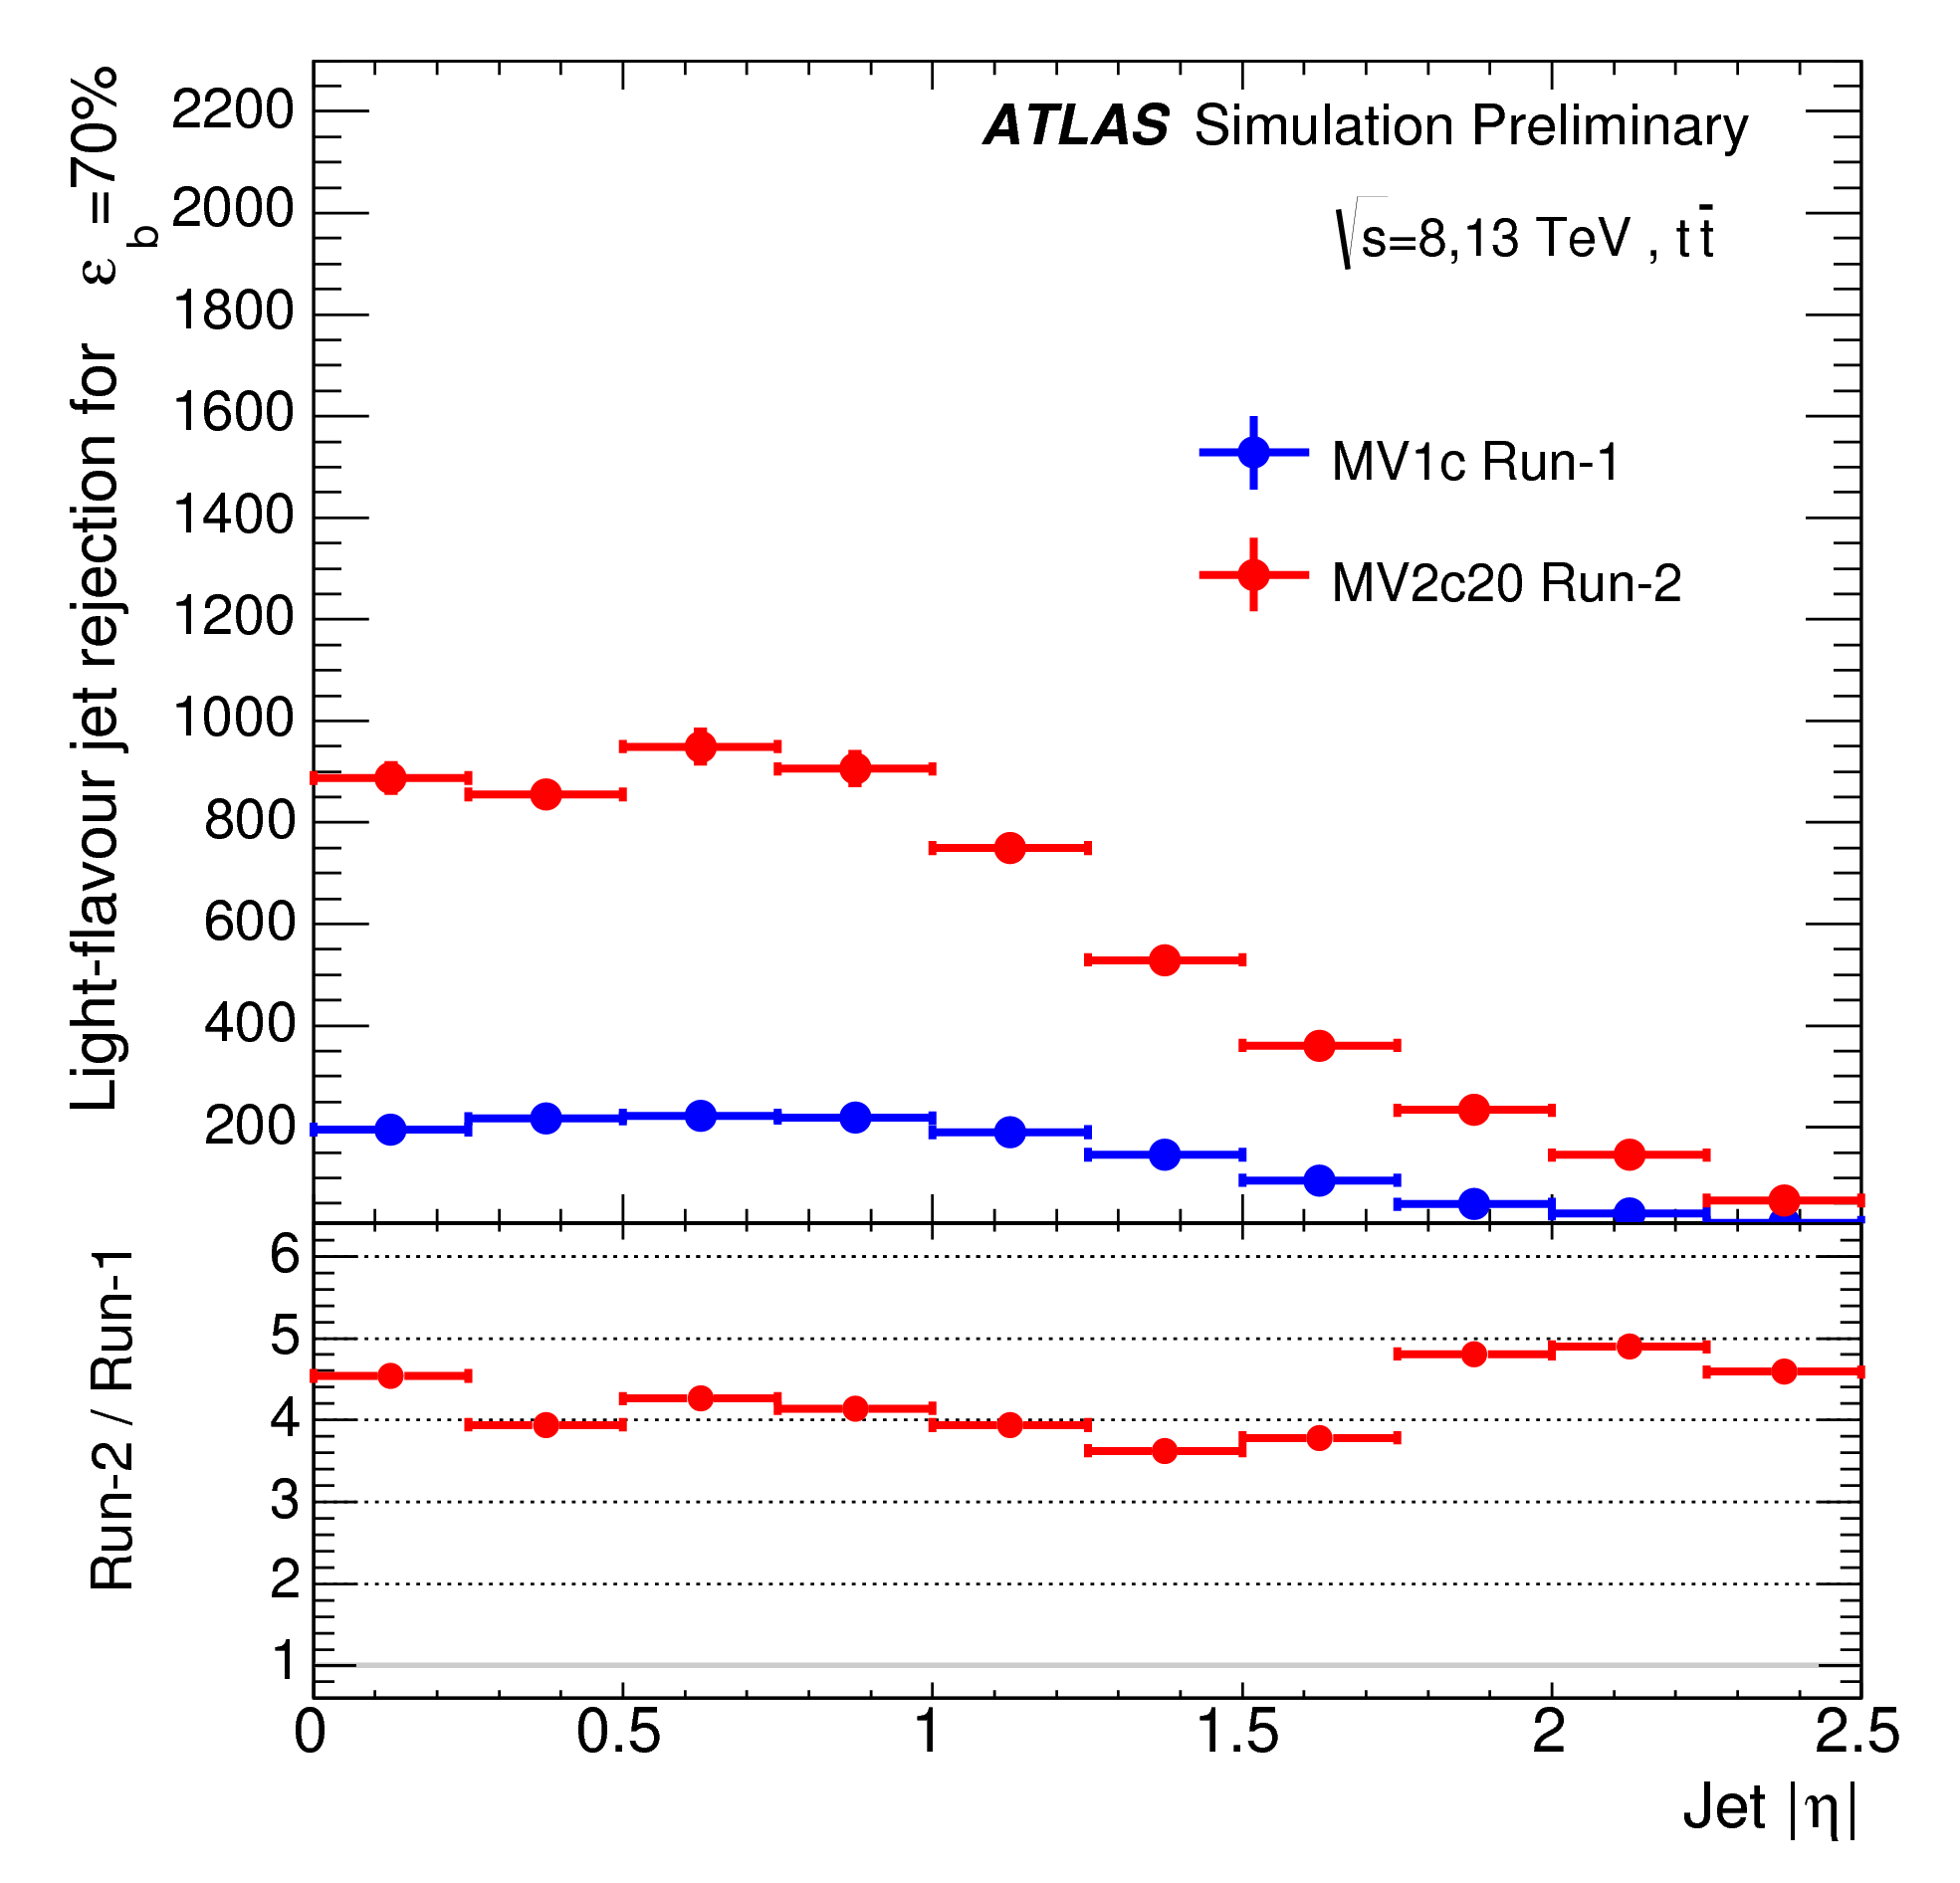
\includegraphics[width=0.5\textwidth]{Images/b-tagging/MV2vsMV1_eta.png}}
\hfill \null
\caption{The light (a) and c-jet rejection (b) versus b-jet efficiency for the MV1c b-tagging algorithm using the \runone detector and reconstruction software (blue) compared to the MV2c20 b-tagging algorithm using the \runtwo setup (red). The light-flavor jet rejection in bins of jet pT (c) and |$\eta$| (d) for the MV1c b-tagging algorithm using the \runone detector and reconstruction software (blue) compared to the MV2c20 b-tagging algorithm using the \runtwo setup (red). In each pT or |?| bin the b-tagging cut value has been chosen in such a way to yield a constant b-jet efficiency of 70\percent.}
\end{figure}
A study over a MonteCarlo sample of $t\overline{t}$ final state have been performed to compare the b-tagging performance in Run1 and at the beginning of Run2.
This requires a comparison to be made between samples produced using the \runone simulation and reconstruction software to those using the \runtwo setup. It is therefore necessary to slightly alter the selection and simulation setup to ensure a meaningful comparison. As opposed to the JVT requirement, the jets are required to be matched to a truth hard-scatter jet. The minimum jet \pt requirement is raised from 20 to 25 GeV. %Additionally the same $t\overline{t}$ sample, but without EvtGen was used, since EvtGen has only been widely used in ATLAS since the start of \runtwo. Not using EvtGen results in a positive shift of about 2 to 3\percent in the b-jet efficiency, when compared to Pythia6 with EvtGen. 
The \runone and \runtwo samples have been produced with different centre of mass energies (8 and 13 TeV) and different pile-up conditions. In order to get an unbiased comparison, the distributions of jet \pt , jet $\eta$ and of the average number of interactions $\mu$ for the \runtwo sample are re-weighted in such a way to reproduce the corresponding \runone distributions.
Figure~\ref{pic:mv2_light} shows the light jet rejection\footnote{light jet rejection is defined as $\frac{1}{\epsilon^l_b}$, where $\epsilon^l_b$ is the efficiency for a light jet to be tagged as a b-jet} respect to the be b-tagging efficiency, for a working point of 70\percent b-tagging efficiency an improvement of factor 4 for the light-jet rejection can be appreciated. Figure~\ref{pic:mv2_c} shows the c-jet rejection\footnote{c-jet rejection is defined as $\frac{1}{\epsilon^c_b}$, where $\epsilon^c_b$ is the efficiency for a c-jet to be tagged as a b-jet} 

\subsection{High pt performances}
The b-tagging algorithm uses MonteCarlo samples as reference to discriminate b-jet from light-jet and c-jet. This happens in the training of the algorithms, in which the flavor of the jet is defined a priori and then the characteristics of each jet family can be recognized. Normally the training is performed with t$\overline{t}$ events samples. This choice is motivated by the decay of the top quark. The only known way that a top quark can decay is through the weak interaction producing a W-boson and a down-type quark (down, strange, or bottom). Because of its enormous mass, the top quark is extremely short-lived with a predicted lifetime of only \SI{5e-25}{\second}\cite{PDG}. As a result top quarks do not have time to form hadrons before they decay, as other quarks do. 
In particular the branching ratio $\Gamma(W+b) / \Gamma(W+q (q = b,s,d))$ = 0.91$\pm$0.04 \cite{PDG}. 
The Standard Model also allows more exotic decays, but only at one loop level, meaning that they are extremely suppressed. For this reason t$\overline{t}$ samples are extremely good to study the b-tagging properties, since most of the time there are at least two b-quarks in the final state, and often associated with light-jet produced in the W decay, which has 69.91$\pm$0.06\% of decaying hadronically.\\


The b-tagging algorithm are trained with t$\overline{t}$ MonteCarlo samples, because of the presence of light-jet and b-jet
The b-tagging performance are typically evaluated over t$\overline{t}$ MonteCarlo samples, because of the presence of light-jet and b-jet. Those
%\subsection{Detector calibration after the insertion}
%\subsubsection{Timing optimization}
%\subsubsection{Chip tuning}
%\subsection{Detector alignment}

